\chapter{Methods}
\label{chap:methods}

%% CONTRIBUTION
\small \paragraph{Contributions} Parts of this chapter are based on the following publication \footnote{with the following author contributions.
Conceptualisation: MK, PDD. Data curation: MK. Formal Analysis: MK. Methodology: MK. Visualisation: MK. Writing – original draft:
MK. Writing – review and editing: MK, PDD, TNP. The contributions of Peter and Tim are highly appreciated.}

\vspace{\baselineskip}
\indent M Klöwer, PD Düben, and TN Palmer, 2020. \emph{Number Formats, Error Mitigation, and Scope for 16-Bit Arithmetics in Weather and Climate Modeling Analyzed With a Shallow Water Model}, \textbf{Journal of Advances in Modeling Earth Systems}, \href{https://doi.org/10.1029/2020MS002246}{10.1029/2020MS002246}.
\vspace{\baselineskip}
\hrule
\vspace{\baselineskip}
\normalsize

This chapter presents the methods that are used in several of the following chapters. We introduce various binary number formats,
their rounding modes, and present error norms to quantify the resulting rounding errors. It follows a section focusing on
programming aspects around type flexibility and code composability to illustrate how custom number formats can be used within
the Julia programming language. The chapter closes with an introduction to information theory to explain the essential concepts
to quantify information in binary number formats.

\section{Binary number formats}
\label{sec:numbers}

This section describes encodings for binary integers (section \ref{sec:integers}), and different formats that approximate real numbers:
Fixed-point numbers (section \ref{sec:fixpoints}), floating-point numbers (section \ref{sec:floats}), logarithmic fixed-point numbers
(section \ref{sec:logfixs}), and posits (section \ref{sec:posits}). A summary on the number formats is given in section \ref{sec:summary_formats}.

\subsection{Integers}
\label{sec:integers}

\subsubsection{Unsigned integers}
\label{sec:uint}

Non-negative integers are represented in binary as unsigned integers. An $n$-bit unsigned integer is a sequence of $n$ bits
$b_1, ..., b_n$ which are decoded into the integer $u$ as a sum of powers of two with exponents $n-1,n-2,...,1,0$
\begin{equation}
	u = \sum_{i=1}^{n} b_i 2^{n-i}
	\label{eq:uint}
\end{equation}
We hereby use the big-endian notation \citep{Cohen1981,James1990}, such that the first bit $b_1$ represents the most significant figure and the last bit $b_n$ the
least significant. For example, the $n=4$ bit unsigned integer \texttt{0101} is decoded as
$0 \cdot 2^3 + 1 \cdot 2^2 + 0 \cdot 2^1 + 1 \cdot 2^0$ and therefore represents the integer $5$ in decimal.

$n$-bit unsigned integers will be referred to as UInt$n$, such that the 8-bit version is called UInt8, and so on. It is often convenient to
write the hexadecimal format to represent unsigned integers or any bit sequence in general. We prefix a hexadecimal with
\texttt{0x}, such that \texttt{1100010010100101} in binary is equivalent to \texttt{0xc4a5} in hexadecimal. Always 4 bits are hereby
grouped and represented with one of the 16 symbols from 0-9 and a-f for the 16 possible states from \texttt{0000} (=\texttt{0x0})
to \texttt{1111} (=\texttt{0xf}). For readability hexadecimal numbers may be intercepted with an underscore, which has no
other meaning, e.g. \texttt{0x5a19\_ab7b = 0x5a19ab7b}.

The range of representable integers with UInt$n$ is 0 to $2^n-1$. Addition, subtraction and multiplication with a result within this
range is exact so that no rounding has to be applied. A result outside this range is in most implementations subject to a \emph{wrap-around}
behaviour which is equivalent to subsequent modulo operation with $2^n$. For example, for UInt16 we have \texttt{0xffff + 0x1 = 0x0}, i.e.
adding 1 to 65536 would return 0; or \texttt{0x0000 - 0x1 = 0xffff}, i.e. subtracting 1 from 0 returns 65536. Such an example of modulo
arithmetic avoids special cases (like NaN for floats, see section \ref{sec:floats}), but can easily yield catastrophic results when integers
are used to approximate real numbers for scientific simulations.

\subsubsection{Signed integers}
\label{sec:int}

While unsigned integers cannot represent negative numbers, signed integers use the first bit $b_1$ to indicate the sign ($b_1 = 0$ is
positive and $b_1 = 1$ negative). One way to decode an $n$-bit signed integer is the sign and magnitude representation
\begin{equation}
	s = (-1)^{b_1}\sum_{i=2}^{n} b_i 2^{n-i-1}
	\label{eq:int}
\end{equation}
which covers the range $[-2^{n-1}-1,2^{n-1}-1]$ but uses two bitpatterns to encode 0 (\texttt{0x00$\dots$00} = +0 and \texttt{0x10$\dots$00} = -0).
However, to avoid multiple representations of zero and to simplify hardware implementations, the sign and magnitude representation
is rarely used. The most common representation uses the two's complement, which flips all bits in a sequence (i.e. \texttt{0 $\to$ 1} and \texttt{1 $\to$ 0})
and adds \texttt{1}. For example, the two's complement of \texttt{0101} is \texttt{1011}. The two's complement representation of negative
integers, i.e. the sign bit is 1, first flips all magnitude bits and then adds $1$ before using Eq. \ref{eq:int} for decoding. For example,
in the 4-bit signed integer format Int4 a value is stored as \texttt{{\color{psign}1}110} (the sign bit is marked in red). The magnitude bits of
\texttt{{\color{psign}1}110} are then converted using the two's complement to \texttt{{\color{psign}1}010} (\texttt{110} is bit flipped into \texttt{001}
and then adding \texttt{1} yields \texttt{010}), which is the sign and magnitude representation (SignMag) that can be decoded using Eq. \ref{eq:int}
into $-2$ in decimal: \texttt{{\color{psign}1}110}$_{\op{Int4}} \to$ \texttt{{\color{psign}1}010}$_{\op{SignMag}} \to -2$. 

Signed integers with the two's complement representation are in $[-2^{n-1},2^{n-1}-1]$, which is subject to a similar wrap-around behaviour 
for arithmetic results beyond the representable range as for unsigned integers. The two's complement representation
is favoured in hardware implementations as no distinction has to be made between signed and unsigned types for the
arithmetic operations addition, subtraction and multiplication \citep{Choo2003}.

\subsection{Fixed-point numbers}
\label{sec:fixpoints}

Fixed-point numbers extend the integer format with fraction bits in order to better approximate real numbers. 
An $n$-bit fixed-point number format uses next to $n_i$ signed integer bits also $n_f$ fraction bits to encode 
an additional sum of powers of two with negative exponents $-1,-2,...,-n_f$. Note that $n = n_i + n_f$, so
every additional fraction bit reduces the number of integer bits. A common notation is, for example,
Q6.10, which is the 16-bit fixed-point format with 6 signed integer bits and 10 fraction bits.
A positive fixed-point number is decoded into $x$ as
\begin{equation}
x = (-1)^{b_1}\sum_{i=2}^{n_i} b_i 2^{n-i-1}  + \sum_{i=1}^{n_f} b_{n_i+i} 2^{-i}
\label{eq:fixpoints}
\end{equation}
The first summation is identical to the signed integers (Eq. \ref{eq:int}), and therefore might use the sign and magnitude
representation as presented here, or the two's complement alternatively. Using $n_f = 1$ can only encode real numbers
at a distance of $\tfrac{1}{2}$ apart, so the representable numbers are $0,\tfrac{1}{2},1,\tfrac{3}{2},2,...$, but using more fraction
bits allows a higher precision. For $n_f=10$ fraction bits, numbers with a spacing of $2^{-10} \approx 0.001$ are representable,
which is also the smallest representable positive number called \emph{minpos}. However, this comes at the cost of a reduced
largest representable number \emph{maxpos} and therefore a smaller range $maxpos-minpos$ (Table \ref{tab:formats}).
For the format Q6.10 with 6 integer bits and 10 fraction bits the largest representable number is $maxpos = \mathtt{0x7fff} = 2^5-1 + \sum_1^{10} 2^{-i}
\approx 31.999$. Results beyond maxpos will trigger in many implementations also a wrap-around behaviour as for integers.

In the following we consider the range of a number format to be $maxpos-minpos$, and the dynamic range as
$\tfrac{maxpos}{minpos}$, usually given in $\log_{10}(\tfrac{maxpos}{minpos})$ orders of magnitude. For a 16-bit fixed-point
number format the range is approximately $2^{n_i-1}$ and therefore decreases with fewer integer bits.
However, the dynamic range is always $2^{n-1}$ and therefore only increases for more bits in an $n$-bit format. For Q6.10
the range is less than $32$ and the dynamic range is 4.5 orders of magnitude.

Choosing the number of integer bits $n_i$ and fraction bits $n_f$ is equivalent to interpreting the bits of a fixed-point number
as an integer with the scaling factor $2^{-n_f}$. Flexibility regarding the range can therefore be achieved with
integer arithmetic if fixed-point numbers are used \citep{Russell2017}. Unfortunately, the very limited range at the cost of precision 
is unsuited for many applications. Nevertheless, they provide exact addition, subtraction and multiplication (as with integers) unless an
overflow or underflow to 0 occurs. They can be suited to represent monetary values for example. However, fixed-point numbers
are rarely used since standardized floating-point numbers became widely available in the 1980s and 1990s.

\subsection{Floating-point numbers}
\label{sec:floats}

While fixed-point numbers have constant accuracy, meaning a fixed number of digits after the decimal point, floating-point
numbers (or simply floats) were introduced for a \emph{floating} decimal point. In consequence, they have an approximately constant
number of significant digits across a wide range of representable numbers. Floating-point numbers achieve this by
encoding an exponent which is multiplied to the significand (also called mantissa).

The floating-point format is standardized in \cite{IEEE1985,IEEE2008} which defines how the bits $b_1,...,b_n$ of an
$n$-bit float are converted into a real number $x$ in terms of a sign bit, $n_e$ exponent and $n_m$ mantissa bits.
Most floats (hence they are called \emph{normal floats}) are decoded as
\begin{equation}
x = (-1)^{sign~bit} \cdot 2^{e-bias} \cdot (1+f)
\label{eq:float}
\end{equation}
and exceptions are discussed in Eq. \ref{eq:float_all}. The exponent bits are interpreted as an unsigned integer $e$, such that $e-bias$ converts
them effectively to signed integers, with $bias = 2^{n_e-1}-1$. Consequently, both positive and negative exponents can be represented,
for absolute values of $x$ larger than 1 and in between 0 and 1, respectively. The bias changes with the number of exponent
bits $n_e$ to have logarithmically a similar range for very large and very small numbers: $e-bias$ is any power of two in
$[-2^{n_e-1}+2,2^{n_e-1}-1]$ for $e=1,...,2^{n_e}-2$. Note, $e=0$ and $e=2^{n_e}-1$ are reserved for special cases such as 0 and infinity,
which will be introduced in Eq. \ref{eq:float_all}.

The mantissa bits $m_1,...,m_{n_m}$ are interpreted as the fraction $f = \sum_{i=1}^{n_m} m_i 2^{-i}$, identical to the fraction bits
of fixed-point numbers (see Eq. \ref{eq:fixpoints}). Including the so-called hidden bit (which represents the addition with $2^0 = 1$
in Eq. \ref{eq:float}) the term $(1+f)$ is in the bounds $[1,2)$, and therefore encodes the significant digits behind the decimal (or binary)
point.

An 8-bit float, for example, encodes the closest float to $\pi = 3.14159...$ with a sign bit (red), $n_e = 3$ exponent bits (blue) and
$n_m=4$ mantissa bits (black) as
\begin{equation}
{\color{psign}0}{\color{pexpo}100}1001_{\op{Float8}} = (-1)^{\color{psign}0} \cdot 2^{{\color{pexpo}4}-bias}
\cdot (1+2^{-1}+2^{-4}) = 3.125 \approx \pi
\label{eq:float8}
\end{equation}
with $bias=2^{n_e-1} - 1 = 3$ here.

In order to also encode 0, plus and minus infinity ($\pm$Inf), and Not-A-Number (NaN), there are exceptions to Eq. \ref{eq:float} that
are discussed in the following: When all exponent bits and mantissa bits are \texttt{0} a float is decoded as 0. If the exponent bits are
all \texttt{0} but the mantissa bits are not ($f>0$) a float is decoded as one of the subnormal numbers, which were introduced to uniformly
fill the gap between 0 and the smallest normal number $2^{-2^{n_e-1}+2}$ (also called \emph{floatmin}) that can be obtained from
Eq. \ref{eq:float}. Another exception to Eq. \ref{eq:float} occurs when all exponent bits are \texttt{1}, in which case the float is decoded
as $\pm \infty$ (depending on the sign bit) if the mantissa bits are all \texttt{0}. However, for any non-zero mantissa bits ($f>0$) the float is
decoded as NaN. In summary,
\begin{equation}
x = \begin{cases}
(-1)^s \cdot 2^{e-bias} \cdot (1+f) \quad &\text{if}~e > 0,\phantom{^{n_e}-1~\text{and}~f > 0} \quad \text{(normals)} \\
(-1)^s \cdot 2^{1-bias} \cdot f \quad &\text{if}~e=0\phantom{^{n_e}-1}~\text{and}~f > 0, \quad \text{(subnormals)} \\
(-1)^s \cdot 0 \quad &\text{if}~e=0\phantom{^{n_e}-1}~\text{and}~f = 0, \quad (\pm 0) \\
(-1)^s \cdot \infty \quad &\text{if}~e=2^{n_e}-1~\text{and}~f = 0, \quad (\pm \text{Inf}) \\
\text{NaN} \quad &\text{if}~e=2^{n_e}-1~\text{and}~f > 0, \quad \text{(Not-A-Number).}
\end{cases}
\label{eq:float_all}
\end{equation}

Floating-point formats cover a wide range of representable numbers. The smallest positive float is called \emph{minpos}, which is the
smallest subnormal number encoded as \texttt{0x00$\dots$01}, $minpos = 2^{2-2^{n_e - 1}-n_m}$. The largest positive float is called
\emph{floatmax} or \emph{maxpos} which occurs for $e=2^{n_e}-2$ (the exponent bits are \texttt{0x11...10}) and 
$f=2-2^{-n_m}$ (the mantissa bits are \texttt{0x11...11}), hence $maxpos = 2^{2^{n_e}-1}\left(1-2^{-n_m-1}\right)$. For an illustration 
of the dynamic range covered by some common floating-point formats see Fig. \ref{fig:methods_decprec_floats}. More exponent
bits allow for a wider dynamic range as both $minpos$ and $maxpos$ effectively scale with $2^{\pm2^{n_e}}$ (positive sign for $maxpos$,
negative sign for $minpos$). However, more exponent bits also mean less mantissa bits which reduces the precision. Consequently,
for a given number of total bits per float there is a trade-off between range and precision, similar to the trade-off for fixed-point numbers.
For more details on the precision of floats see section \ref{sec:decimal_precision}.

Due to the exponent bits floats are approximately logarithmically distributed on the real number line with about half of the representable
numbers packed between -1 and 1. However, due to the mantissa bits being a sum of powers of two with negative exponents floats
are also piecewise uniformly (or linearly) distributed. Within a given range of two powers of two $[2^i,2^{i+1})$, e.g. $[1,2)$ or
$[\tfrac{1}{8},\tfrac{1}{4})$ only the mantissa bits change, such that the distance $\delta$ between two subsequent 
floats is always equal and $\delta = 2^{i-n_m}$. But for the next larger power of two, this distance doubles, whereby
this doubling accounts for the approximately logarithmic distribution of floats throughout the dynamic range. The distance $\delta$ is
closely related to the rounding error and discussed in more detail in section \ref{sec:roundnearest}.

The two most common floating-point formats are Float32 and Float64. Float32 is a 32-bit format with $n_e=8$ exponent bits and
$n_m=23$ mantissa bits. Float64 is a 64-bit format with $n_e=11$ exponent bits and $n_m=52$ mantissa bits. Both have been 
standardized in \cite{IEEE1985}. Recently more widely available on specialised hardware are the two 16-bit low precision formats
Float16 (5 exponent bits and 10 mantissa bits) and BFloat16 (8 exponent bits and 7 mantissa bits, a truncated version of Float32).
The number $\pi = 3.14159...$ is encoded in these formats as (sign bit in red, exponent bits in blue, mantissa bits in black)
\begin{align}
\text{Float64:}& \quad {\color{psign}0}{\color{pexpo}10000000000}10010010000111111011 \nonumber \\
			& \quad 01010100010001000010110100011000 = 3.141592653589793 \nonumber \\
\text{Float32:}& \quad {\color{psign}0}{\color{pexpo}10000000}10010010000111111011011 = 3.1415927 \nonumber \\
\text{Float16:}& \quad {\color{psign}0}{\color{pexpo}10000}1001001000 = 3.140625 \nonumber \\
\text{BFloat16:}& \quad {\color{psign}0}{\color{pexpo}10000000}1001001 = 3.140625
\end{align}
While both Float16 and BFloat16 represent $\pi$ as 3.140625 note that Float16 is three bits more precise, which just happen to be all \texttt{0}.

Floating-point formats have many ways to encode a NaN (Eq. \ref{eq:float_all}). In the case of the exponent bits being all \texttt{1} any non-zero
mantissa encodes a NaN, which amounts to $2^{n_m+1}-2$ possibilities ($2^{n_m+1}$ for all combinations of mantissa bits and the sign,
minus two for the mantissa being zero, which encodes $\pm$Inf). Hence, for Float64 there are more than $1.8 \cdot 10^{16}$ bitpatterns
that encode NaN, which are, however, only $2^{-n_e} \approx 0.05\%$ of all bitpatterns. Despite fewer mantissa bits, for Float16 there are
still 2046 ways to encode a NaN, about $3.1\%$ of all available bitpatterns (see also Fig. \ref{fig:a64fx_bitpatternhist}).

A summary of the characteristic of different floating-point formats is found in Table \ref{tab:formats}. For a more in-depth discussion of
the precision of these formats see section \ref{sec:decimal_precision}.

\subsection{Logarithmic fixed-point numbers}
\label{sec:logfixs}

The major difference between floats and integers (or fixed-point numbers) is their ability to represent very large and very small
numbers simultaneously at similar precision. The floating-point format achieves this with exponent bits such that the floats are
approximately logarithmically spaced out on the positive and negative part of the real number line. This motivates us to define
a logarithmic fixed-point number format (in short logfix), which is not a hybrid format of linear and logarithmic spacing as floats are, but
follows a perfect logarithmic spacing. We implement the logfix formats presented here as the software emulator 
\href{https://github.com/milankl/LogFixPoint16s.jl}{LogFixPoint16s.jl} and further technical details can be found therein.

Logfixs are an appealing number format as multiplication, division, square root and power are exact and do not include any rounding
errors unless the result is outside the representable range. This property is equivalent to fixed-point numbers being exact
on addition and subtraction, which, due to the logarithm, translates to multiplication and division for logfixs. We design an $n$-bit logfix
format with one sign bit $s$, and in the exponent $n_i$ signed integer bits followed by $n_f$ fraction bits,
such that $n = 1 + n_i + n_f$. The decoding of a logfix number is defined as
\begin{equation}
x = (-1)^{b_1} \cdot 2^k
\label{eq:logfix}
\end{equation}
with the exponent $k = i + f$ being a fixed-point number with $n_i$ integer bits and $n_f$ fraction bits. The signed integer $i$
is in $[-2^{n_i-1},2^{n_i-1}-1]$ (one bit is effectively used for the sign of the exponent) and uses a biased representation similar
to floats: The integer bits are first interpreted as an unsigned integer $u$ and converted to the signed integer $i$ by $i = u - bias$,
where $bias = 2^{n_i-1}$. For example, with $n_i = 5$ integer bits the bitpattern $u = \mathtt{10001} =  17$ is converted as
$i = u - bias = 17-2^4 = 1$, such that for $f=0$ the logfix \texttt{01000100$...$} represents the number 2. The fraction $f$
is in $[0,1)$ and identical to the mantissa encoding in floating-point numbers (but without the hidden bit)
$f = \sum_{i=1}^{n_f} b_{1+n_i+i} 2^{-i}$.

Eq. \ref{eq:logfix} has only two exceptions: The bit pattern \texttt{00$\dots$00} is reserved to encode zero and \texttt{100$\dots$0}
to encode Not-A-Real (NaR, which combines NaN with $\pm \infty$ into a single bitpattern and is borrowed from the design of
posits, see section \ref{sec:posits}). Hence, $x=0$ if $b_1 = k = 0$ and $x = \text{NaR}$ if $b_1 = 1$ but $k=0$.

The trade-off between precision and range is for logfixs similar to floats when choosing a corresponding number of bits:
The logfix format with $n_i=5$ integer bits and $n_f=10$ fraction bits is similar to Float16 with 5
exponent bits and 10 mantissa bits. Using $n_i=8$ integer bits and $n_f=7$ fraction bits is similar to BFloat16, such that
we call these two logfix formats LogFixPoint16 and BLogFixPoint16 in analogy. The smallest representable positive number
for logfixs is $minpos = 2^{-2^{n_i-1} + 2^{-n_f}}$ which is encoded as \texttt{00$...$01}. The largest representable number
for logfixs is $maxpos = 2^{2^{n_i-1} - 2^{-n_f}}$ encoded as \texttt{011$...$1}, such that for our design of logfixs
$maxpos = \tfrac{1}{minpos}$, meaning that the dynamic range is symmetric around 1. This is not the case for floats,
as special cases like NaNs occupy part of the theoretically available dynamic range (see Eq. \ref{eq:float_all}).
Logfixs are therefore symmetric with respect to the multiplicative inverse around 1 and symmetric with respect to addition
around 0. Floats are only symmetric with respect to addition.

Multiplication, division, square root and power are easily implemented for a logarithmic number format with integer arithmetic. 
Multiplication of two numbers $x,y$, for example, is equivalent to the addition of the exponents
\begin{equation}
xy = (-1)^{s_x \veebar s_y} \cdot 2^{k_x + k_y}
\label{eq:logfix_mul}
\end{equation}
with $\veebar$ being the logical xor-operation on the sign bits $s_x,s_y$. Exceptions to Eq. \ref{eq:logfix_mul} occur for $x = \text{NaR}$
or $y = \text{NaR}$ in which case $xy = \text{NaR}$, or if no NaRs are present but if $x=0$ or $y=0$ then $xy= 0$. The multiplication 
is then followed by checking for underflows ($xy < \tfrac{1}{2}minpos$) or overflows ($xy > maxpos$), in which case 0 or NaR is returned,
respectively. 

Addition and subtraction for logfixs is based on the Gaussian logarithms $G^+,G^-$ which are functions of the argument $a$
\begin{align}
G^+(a) = -a + \log_2(1+2^a) \nonumber \\
G^-(a) = -a + \log_2(1-2^a)
\label{eq:gauss_log}
\end{align}
The evaluation of the Gaussian logarithms makes addition and subtraction for logfixs much more complicated than the other arithmetic operations.
The result $z = (-1)^{s_z} \cdot 2^{k_z}$ of an addition $x+y = z$ is given by
\begin{align}
k_z &= \log_2(\vert x \vert + \vert y \vert) \nonumber \\
	&= k_y - (k_y - k_x) + \log_2(1+2^{k_y - k_x})  = k_y + G^+(k_y-k_x)
\label{eq:logfix_add}
\end{align}
and similar for subtraction $y-x = z$
\begin{align}
k_z &= \log_2(\vert y \vert - \vert x \vert) \nonumber \\
	&= k_y - (k_y-k_x) + \log_2(1-2^{k_y - k_x}) = k_y + G^-(k_y-k_x)
\label{eq:logfix_sub}
\end{align}
for $y \geq x \geq 0$, which can be generalised to all $x,y$ by rewriting $x+y$ as $y+x$ or $x-y = -(y-x)$, etc.

The result of the base-2 logarithm $\log_2$ inside the Gaussian logarithms has to be rounded to a fixed-point
number like $k_x$ and $k_y$ for the subsequent addition. Consequently, for any finite-precision logfix format
the Gaussian logarithms become
\begin{align}
	G^+(a) = -a + \op{round}(\log_2(1+2^a)) \nonumber \\
	G^-(a) = -a + \op{round}(\log_2(1-2^a))
	\label{eq:gauss_log_round}
\end{align}
which introduces a rounding error in general, meaning that addition and subtraction with logfixs are not exact.
We will discuss rounding for logfixs in section \ref{sec:roundnearest_logfix}, and define the specific rounding function
round() therein.

Instead of evaluation the Gaussian logarithms on every arithmetic operation, they can be precomputed as only a function of the single argument
$k_y-k_x$. For an $n$-bit logfix format there are only $2^{n-1}-1$ different values for $k_y-k_x$, such that in 16 bit the two precomputed table
lookups have an upper bound of $32767$ entries each. In practice, such table lookups are considerably smaller as for $k_y \gg k_x$  the functions
$G^+,G^-$ approach zero, as their increment on $k_y$ is eventually round back to $k_y$. Consequently, there will be a maximum resolvable
difference $k_y-k_x$ beyond which $G^+$ and $G^-$ do not have to be computed. For the $n=16$-bit format LogFixPoint16 with $n_f=10$
fraction bits the two table lookups are each 24KB large (11805 entries at 16 bit per entry). For BLogFixPoint16 ($n_f=7$ fraction bits) the two
table lookups are even smaller at 2KB each (1092 entries at 16 bit per entry). While the small sizes of these table lookups are promising
for low-precision hardware implementations, addition and subtraction remain the performance and precision bottleneck for logfix
formats. The size of these table lookups increases exponentially with the number of bits, meaning that implementations
for 32-bit or 64-bit logfixs cannot be based on table lookups. Such high-precision logfix formats will only be possible
if the logarithms can be computed directly.  Although the design of floats is mathematically more complicated
(compare Eq. \ref{eq:float_all} to Eq. \ref{eq:logfix}), they enjoy full hardware support, such that there's currently no 
competitive hardware based on logfix arithmetic available that could be used as an alternative to floats.

For a summary on the logfix formats LogFixPoint16 and BLogFixPoint16 see section \ref{sec:summary_formats} and Table \ref{tab:formats}.

\begin{figure}[tbhp]
	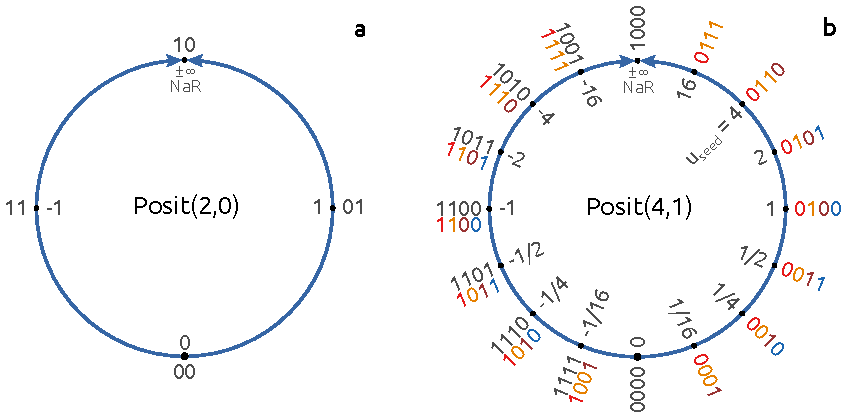
\includegraphics[width=1\textwidth]{Figures/methods/posit_circles.pdf}
	\caption{\textbf{Two posit number formats obtained by projecting the real axis onto a circle.}
	\textbf{a} The 2-bit Posit(2,0) format and \textbf{b} the 4-bit Posit(4,1) format. The bitpatterns are marked on the outside
	and the respective values on the inside of each circle. Bit patterns of negative numbers (black) have to be converted to their
	two's complement (colours) first. At the top (12 o'clock) of every posit circle is Not-A-Real (NaR), also called complex infinity ($\pm \infty$),
	at the bottom (6 o'clock) is always 0, at 3 o'clock always 1 and at 9 o'clock always -1. After \cite{Gustafson2017a}.}
	\label{fig:posit_circle}
\end{figure}

\subsection{Posit numbers}
\label{sec:posits}

Posit numbers were introduced by \cite{Gustafson2017a} as one of the universal number formats (Unums, \cite{Gustafson2015})
and arise from a projection of the real axis onto a circle (Fig. \ref{fig:posit_circle}).
With only one bitpattern for 0 and one for Not-a-Real (NaR, or complex infinity $\pm \infty$, a replacement for Not-a-Number NaN),
posits have a bijective mapping between all available bitpatterns and representable numbers. The circle is split into
\emph{regimes}, determined by a constant $useed$, which always marks the north-west on the posit circle (Fig. \ref{fig:posit_circle}b).
Regimes are defined by $useed^{\pm1}$, $useed^{\pm2}$, $useed^{\pm3}$, etc. To encode these regimes into bits, posit
numbers extend floating-point arithmetic by introducing regime bits that are responsible for the dynamic range of representable
numbers. Instead of having a fixed length, regime bits are defined as the sequence of identical bits after the sign bit, which are
eventually terminated by an opposite bit, e.g. \texttt{000001} or \text{1110}, the last bit is the terminating bit respectively.

The flexible length allows the mantissa (or significand) to occupy more bits when less regime bits are needed, which is the
case for numbers around 1 and -1 (in a logarithmic sense). More mantissa bits mean a that the representable numbers are
denser packed, resulting in a higher precision around $\pm 1$. On the other hand, the regime bits occupy more bit positions
for very small or very large numbers in an absolute sense, e.g. $-10^{-10}$ or $10^{10}$, which reduces the number of 
available mantissa bits for those. Therefore, the higher precision around $\pm 1$ for posits is traded against a gradually
lower precision for very small or very large numbers. While floats have a constant number of mantissa bits such that
the result of a calculation is always precise to a similar amount of significant digits, calculations with posits will be more precise
when the result is around $\pm 1$. Depending on the application, this can reduce rounding errors. For a quantitative comparison
of the precision of the number formats see section \ref{sec:decimal_precision}.

A number is encoded into an $n$-bit posit with a sign bit $s$, $n_r$ regime bits including the terminating bit, up to $n_e$ exponent bits
and $n_m$ mantissa bits, such that $n = 1 + n_r + n_e + n_m$. A posit format is uniquely defined by the number of bits $n$
and the number of exponent bits $n_e$ and we call this format Posit($n$,$n_e$). However, as illustrated in Fig. \ref{fig:posit_circle}
for the format Posit(4,1) with one exponent bit, the regime bits can occupy as many bit positions such that the exponent bits
are pushed beyond the available bit positions. In this case there are actually less than $n_e$ exponent bits explicitly encoded,
and the hidden exponent bits are implicitly assumed to be \texttt{0}. The same holds for the mantissa bits, which are all
implicitly \texttt{0} if no bit positions are available for the mantissa.

For positive numbers, decoding from posit bits into the number $p$ is defined as
\citep{Gustafson2017a,Klower2019a,Chen2018} (negative posits are converted first to their two's complement, see
Eq. \ref{eq:2comp})
\begin{equation}
p = (-1)^s \cdot useed^k \cdot 2^e \cdot (1+f)
\label{eq:posit}
\end{equation}
where $k$ is the number of regime bits excluding the terminating bit. $e$ is the unsigned integer represented by the
exponent bits and $f$ is the fraction which is encoded in the fraction (or mantissa) bits. The base $useed = 2^{2^{n_e}}$ is
determined by the number of exponent bits $n_e$ in a given format, e.g. for Posit(4,1) $useed = 4$. More exponent bits
increase - by increasing $useed$ - the dynamic range of representable numbers at the cost of precision,
as increasing $useed$ also increases the spacing between representable numbers. The exponent bits themselves do
not affect the dynamic range by changing the value of $2^e$ in Eq. \ref{eq:posit}. Instead, they fill gaps of
powers of two spanned by $useed = 4,16,256,...$ for $n_e=1,2,3,...$, such that the regime and exponent combined
encodes every power of two over the range of representable numbers. Hence, every posit number can be written as
$p = \pm 2^n \cdot (1+f)$ with a given integer $n$ \citep{Gustafson2017a,Chen2018}. The mantissa bits encode the
fraction $f$ following the floating-point standard \citep{IEEE1985}, see section \ref{sec:floats}, with the difference that
the number of mantissa bits $n_m$ can change.

An example for posit decoding is provided in the Posit(8,1)-system (i.e. $useed = 4$)
\begin{equation}
57 \approx \mathtt{{\color{psign}0}{\color{pregime}111}{\color{pregimet}0}{\color{pexpo}1}11}_{\op{Posit}(8,1)} = (-1)^{\color{psign}0}
\cdot 4^{\color{pregime}2} \cdot 2^{\color{pexpo}1} \cdot (1+2^{-1}+2^{-2}) = 56
\label{eq:posit_pos}
\end{equation}
The sign bit is given in red, regime bits in orange, the terminating regime bit in brown, the exponent bit in blue and the fraction bits in black.
The $k$-value is inferred from the number of regime bits, that are counted as negative for the regime bits being \texttt{0}
(which encodes numbers $\vert p \vert <1$), e.g. \texttt{{\color{pregime}000}{\color{pregimet}1}} yields $k=-3$. For the regime bits being \texttt{1}
they are counted as positive but subtract 1 (which encodes numbers $\vert p \vert \geq 1$), e.g. \texttt{{\color{pregime}111}{\color{pregimet}0}}
yields $k=2$.

For negative numbers, i.e. the sign bit being $s=1$, all other bits are first converted to their two's complement (flipping all bits and adding \texttt{1}, 
see section \ref{sec:int} and \cite{Choo2003}), denoted here with an underscore subscript
\begin{equation}
\begin{split}
-0.28 &  \approx \mathtt{11011110}_{\op{Posit}(8,1)} = \mathtt{{\color{psign}1}{\color{pregime}0}{\color{pregimet}1}{\color{pexpo}0}0010}\_ \\
& = (-1)^{\color{psign}1} \cdot 4^{\color{pregime}-1} \cdot 2^{\color{pexpo}0} \cdot (1+2^{-3}) = -0.28125.
\end{split}
\label{eq:2comp}
\end{equation}
After the conversion to the two's complement, the bits are interpreted in the same way as in Eq. \ref{eq:posit_pos}. Posits have two exceptions.
The bitpattern \texttt{00$...$00} is reserved to represent 0 and the bitpattern \texttt{100$...$0} represents Not-a-Real (NaR). Many functions
are simplified for posits, as only these two exceptions cases have to be handled. Conversely, Float64 has more than
$10^{15}$ bitpatterns reserved for NaN. Although they only make up $< 0.05\%$ of all available bit patterns, the percentage of redundant
bitpatterns for NaN increases for floats with fewer exponent bits (Table \ref{tab:formats}), and only poses a noticeable issue for Float16
and Float8.

The smallest representable number $minpos$ for posits is encoded in the bitpattern \texttt{{\color{psign}0}{\color{pregime}00...0}{\color{pregimet}1}}
(Fig. \ref{fig:posit_circle}b), with $n-2$ regime bits, such that $k = -(n-2)$ and $minpos = useed^k = 2^{-2^{n_e}(n-2)}$. Posits are symmetric with respect
to the multiplicative inverse around 1 and therefore the largest representable number $maxpos =  \tfrac{1}{minpos}$, which occurs for 
the bitpattern \texttt{{\color{psign}0}{\color{pregime}11...1}}, with $n-1$ regime bits, such that $k=n-2$ and $maxpos = useed^k = 2^{2^{n_e}(n-2)}$,
as required for symmetry. Posits also come with a no-overflow rounding mode, which will be discussed in more detail
in section \ref{sec:roundnearest}.

The proposed posit standard defines several posit number formats as a drop-in replacement for floats. Posit8 is the 8-bit posit format with 0
exponent bits (hence also called Posit(8,0)). Although 8-bit floats are not officially defined, the Float8 format presented in Table \ref{tab:formats}
has 3 exponent bits and has a similar range-precision trade-off as Posit8. Posit16 is the 16-bit format with 1 exponent bit, hence also called
Posit(16,1) and is thought to be the alternative to Float16. Posit32 is the 32-bit posit format with 2 exponent bits, hence shortened from
Posit(32,2), which is proposed to be the alternative to Float32. The following chapters will mostly investigate Posit8,Posit16 and Posit32,
as in the proposed posit standard, but chapter \ref{chap:shallow_water} will additionally discuss Posit(16,2).

The posit number framework also highly recommends \emph{quires}, an additional register on hardware to store intermediate results.
Dot-product operations are fused with quire arithmetic and can therefore be executed with a single rounding error, which is only applied
when converting back to posits. The quire concept could also be applied to floating-point arithmetic (fused multiply-add is available on
some processors), but is technically difficult to implement on hardware for a general dot-product as the required registers would need
to be much larger in size. For fair comparison we do not take quires into account. 

In order to use posits on a conventional CPU we developed for the programming language Julia \citep{Bezanson2017} the posit
emulator \emph{SoftPosit.jl} \citep{Klower2019}, which is a wrapper for the C-based library SoftPosit \citep{Leong2020}.

\subsection{Summary on number formats}
\label{sec:summary_formats}

\begin{table}[htbp]
	\center
	\begin{tabular}{l | r | r | l | l | r | r | r}
	\textbf{Format} & bits & exp bits & $minpos$ & $maxpos$ & dyn range & $\epsilon$ &  \% NaR \\
	\hline
	Float64    & $64$ & $11$ & $5.0 \cdot 10^{-324}$ & $1.8 \cdot 10^{308}$ & 631.6 & $16.3$ & $0.0$ \\
	Float32    & $32$ & $8$ & $1.0 \cdot 10^{-45}$ & $3.4 \cdot 10^{38}$ & 83.4 & $7.6$ & $0.4$ \\
	Float16    & $16$ & $5$ & $6.0 \cdot 10^{-8}$ & $65504$ & 12.0 & $3.7$ & $3.1$ \\
	BFloat16    & $16$ & $8$ & $ 9.2 \cdot 10^{-41}$ & $3.4 \cdot 10^{38}$ & 78.6 & $2.8$ & $0.4$  \\
        Float8 & $8$ & $3$ & $1.5 \cdot 10^{-2}$ & $15.5$ & 3.0 & $1.9$ & $12.5$\\
        \hline
        Posit32 & $32$ & $2$ &  $7.5 \cdot 10^{-37}$ & $1.3 \cdot 10^{36}$ & 72.2 & $8.8$ & $0.0$ \\
        Posit16 & $16$ & $1$ & $3.7 \cdot 10^{-9}$ & $2.7 \cdot 10^{8}$ & 16.9 & $4.3$ & $0.0$\\
        Posit(16,2) & $16$ & $2$ & $1.4 \cdot 10^{-17}$ & $7.2 \cdot 10^{16}$ & 33.7 & $4.0$ & $0.0$\\
        Posit8 & $8$ & $0$ & $1.6 \cdot 10^{-2}$ & $64$ & 3.6 & $2.2$ & $0.4$  \\
        \hline
        Int64 & $64$ & $0$ & $1$ & $9.2 \cdot 10^{18}$ & 19.0 & $0.8$ & $0$\\
        Int16 & $16$ & $0$ & $1$ & $32767$ & 4.5 & $0.8$ & $0$\\
        Q6.10 & $16$ & $0$ & $9.8 \cdot 10^{-4}$ & $32.0$ & 4.5 & $3.7$ & $0$\\
        \hline
        LogFixPoint16 & $16$ & $5$ & $1.5 \cdot 10^{-5}$ & $65491.7$ & 9.6 & $3.8$ & $0.0$\\
        BLogFixPoint16 & $16$ & $8$ & $5.4 \cdot 10^{-20}$ & $9.1 \cdot 10^{18}$ & 77.1 & $2.9$ & $0.0$
        \end{tabular}
        \vspace{10pt}
	\caption{\textbf{Some characteristics of various number formats.} The number of exponent bits is for logfixs the number of
	integer bits in the exponent (see section \ref{sec:logfixs}). $minpos$ is the smallest representable positive number,
	$maxpos$ the largest. The dynamic range is $\log_{10}(\tfrac{maxpos}{minpos})$. The machine precision $\epsilon$ is the decimal
	precision at $1$ (see section \ref{sec:decimal_precision}), equivalent to the decimal places at least correct after rounding.
	\% NaR denotes the percentage of bit patterns that represent Not-A-Number (NaN), infinity or Not-A-Real (NaR).}
	\label{tab:formats}
\end{table}

Some characteristics of the presented binary number formats are summarized in Table \ref{tab:formats}. Integer formats are usually
unsuited for scientific computing as no numbers between 0 and 1 can be represented. While fixed-point numbers can act as
scaled integers, this lowers $maxpos$ as the dynamic range $\log_{10}(\tfrac{maxpos}{minpos})$ does not change between signed
integers and fixed-point numbers, and is comparably small. Floating-point numbers are therefore in general a much better
choice for scientific computing as they provide a large dynamic range as a sufficiently high precision around 1. Virtually equivalent
to floats in these characteristics are logarithmic fixed-point numbers, which also avoid a large share of NaRs in their design.
Following these characteristics, posits are slightly superior to floats and logfixs with the same number of bits. A more in-depth
comparison of these number formats is part of chapter \ref{chap:orbits} and \ref{chap:shallow_water}.

\section{Rounding modes}
\label{sec:rounding}

Representing a real number $x$ in any finite-precision number format introduces, in general, a rounding error (or round-off error) as
only an approximation to $x$ can be represented in a given format. Depending on the distribution of the representable numbers on the
real axis the rounding error will differ and in the case where $x$ is exactly representable no rounding error occurs. Such rounding errors
occur in the conversion between formats, but in general also after arithmetic operations within one format, including two argument
operations such as addition and multiplication but also single-argument operation such as the square root. Rounding errors arise when
the arithmetic result does not map again onto a representable number. For example, $1+1 = 2$ results in another integer that is again
representable within the format, hence no rounding is applied. However, $5/4 = 1.2$ and the result is not representable as integer.
Therefore rounding has to be applied to make the result representable again, introducing a rounding error. The set of rules that decide
which representable number serves as approximation to the exact result is called the rounding mode.

Rounding a number in a given format usually makes its representation simpler by some measure. For example, rounding $\pi = 3.14159...$
to $3.1$ reduces the number of decimal places required to represent an approximation to $\pi$. However, the representation is usually
only simplified in the format where the rounding is applied in: While the approximation $3.1$ of $\pi$ requires less decimal places (meaning
that trailing decimal places are set to zero) its representation in Float32 does not necessarily set any number of trailing bits to zero
\begin{align}
\text{Float32:}& \quad \mathtt{{\color{psign}0}{\color{pexpo}10000000}10010010000111111011011} = 3.1415927 \nonumber \\
\text{Float32:}& \quad \mathtt{{\color{psign}0}{\color{pexpo}10000000}10001100110011001100110} = 3.1 \nonumber \\
\text{BFloat16:}& \quad \mathtt{{\color{psign}0}{\color{pexpo}10000000}1001001} = 3.140625
\end{align}
However, as shown in this example, rounding in binary from Float32 to BFloat16 sets trailing bits to zero, but does not considerably
reduce the decimal places. In the following we will present several \emph{binary} rounding modes, meaning that the binary encoding
of an exact value within a given format is replaced by shorter (or at least simpler due to more trailing zeros) bit sequence, representing
an approximation to the exact value.

\begin{figure}[tbhp]
	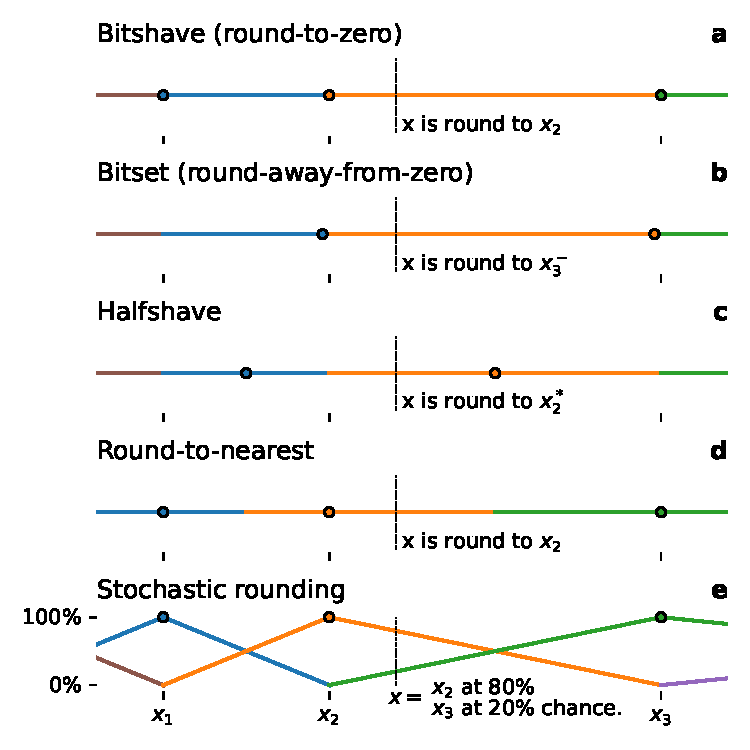
\includegraphics[width=1\textwidth]{Figures/methods/rounding_modes.pdf}
	\caption{\textbf{Schematic to illustrate some rounding modes. a}
	Bitshave rounds the exact value $x$, indicated by a dashed line, down to the next smaller or equal representable number $x_2$. \textbf{b}
	Bitset rounds $x$ up to $x_3^- = x_3-\epsilon$, i.e. just smaller than $x_3$ by machine precision $\epsilon$ of the exact representation
	(see Eq. \ref{eq:bitset}). \textbf{c} Halfshave rounds $x$ to $x_2^* = \tfrac{x_2 + x_3}{2}$ which is half-way between the representable
	numbers $x_2,x_3$. \textbf{d} Round-to-nearest rounds $x$ to the nearest representable number, $x_2$ here. Nearest is hereby defined
	as the smallest linear distance $\vert x - x_i \vert$ for all representable numbers $x_i$. \textbf{e} Stochastic rounding rounds $x$ up or
	down at a chance that is proportional to the distance of $x$ with its adjacent representable numbers. Here, $x$ is located one fifth the
	way between $x_2$ and $x_3$, hence it is round down to $x_2$ in $1-\tfrac{1}{5} = 80\%$ of the cases, but round up to $x_3$ at
	$\tfrac{1}{5} = 20\%$ chance. The rounding modes \textbf{a}-\textbf{d} are deterministic. Line segments and representable numbers
	(circles) are colour-coded, such that the all numbers on a line segment of a given colour are rounded to the representable number
	with the same colour.}
	\label{fig:methods_rounding_modes}
\end{figure}

\subsection{Bitshaving, bitsetting and halfshave}
\label{sec:bitshave}

Bitshave is one of the simplest binary rounding modes that \emph{shaves} off a given amount of trailing bits and sets them to \texttt{0}
\citep{Zender2016,Kouznetsov2020}. This is the binary version of \emph{round-to-zero}, which rounds down for positive values, but
rounds up for negative values. For an exact value $x$ in between two representable numbers $x_1,x_2$ round-to-zero is
\begin{equation}
	\op{round}_{\op{to-zero}}(x) = \begin{cases} x_1, \quad \text{if } x \geq 0 \text{ and } x_1 \leq x < x_2 \\
									x_2, \quad \text{if } x < 0 \text{ and } x_1 < x \leq x_2 \end{cases}
	\label{eq:round_zero}
\end{equation}
For an illustration of the round-to-zero see Fig. \ref{fig:methods_rounding_modes}a. The binary version bitshave achieves this behaviour
by setting trailing mantissa bits to 0, which reduced the fraction $f$ in the mantissa
(Eq. \ref{eq:float}). For example, bitshaving $\pi$ in Float32 to 7 mantissa bits yields (rounded bits in grey)
\begin{align}
	\text{Float32:}& \quad \mathtt{{\color{psign}0}{\color{pexpo}10000000}10010010000111111011011} = 3.1415927 \nonumber \\
	\text{Float32, bitshaved:}& \quad \mathtt{{\color{psign}0}{\color{pexpo}10000000}1001001{\color{gray}0000000000000000}} = 3.140625
	\label{eq:bitshave}
\end{align}
This rounding mode therefore introduces a worst-case error that is equivalent to $\delta = x_2-x_1$, the distance between the two
representable numbers. The worst-case error occurs if the trailing bits that are subject to rounding are all \texttt{1}, which means
that the exact value $x$ is just smaller (for positive $x$) than a representable number. For example, bitshaving $x = \mathtt{0111}$
to one leading bit yields $x_1 = \mathtt{0{\color{gray}000}}$, although the next larger representable number $x_2 = \mathtt{1000}$
is closer to $x$.

Bitshave is a rounding mode with a bias towards zero: For positive numbers, it will always round to values that are smaller or the
same, therefore it is expected to reduce the mean. For numbers of either sign, bitshave will reduce the variance, as it will always
round to values that are closer to zero or the same.

\subsubsection{Bitset}
An alternative to bitshaving is bitsetting \citep{Zender2016}, which sets the trailing bits to \texttt{1} instead. Following the same
example as above (Fig. \ref{fig:methods_rounding_modes}b)
\begin{align}
	\text{Float32:}& \quad \mathtt{{\color{psign}0}{\color{pexpo}10000000}10010010000111111011011} = 3.1415927 \nonumber \\
	\text{Float32, bitset:}& \quad \mathtt{{\color{psign}0}{\color{pexpo}10000000}1001001{\color{gray}1111111111111111}} = 3.1562498
	\label{eq:bitset}
\end{align}

Different to bitshave, bitsetting has a bias away from zero and will increase the variance following similar arguments. Furthermore,
although the trailing bits are simpler because they are all \texttt{1}, they still have to be explicitly stored to preserve the rounded
value. So while bitsetting is a valid binary rounding mode, it does not provide any storage benefits and will need to be combined
with methods like lossless compression (see section \ref{sec:compression_methods_compression}) to actually yield rounded
values that require fewer bits in memory.

\subsubsection{Halfshave}
To remove the biases from bitshaving and bitsetting, the binary rounding mode halfshave is proposed \citep{Zender2016,Kouznetsov2020}.
This rounding mode is similar to bitshaving, but replaces the shaved bits with \texttt{1000$...$} instead of \texttt{0000$...$}.
Halfshave therefore replaces the representable numbers $x_1,x_2,x_3,...$ from bitshaving with the respective mid-points.
Halfshaved representable numbers are therefore $x_1^* = \tfrac{x_1+x_2}{2}, x_2^* = \tfrac{x_2 + x_3}{2}, ...$ and require
one more bit (which is always \texttt{1}) to be stored explicitly (which can be subject to lossless compression due to redundancy,
see section \ref{sec:compression_methods_compression}). Following the same example as above
\begin{align}
	\text{Float32:}& \quad \mathtt{{\color{psign}0}{\color{pexpo}10000000}10010010000111111011011} = 3.1415927 \nonumber \\
	\text{Float32, bitset:}& \quad \mathtt{{\color{psign}0}{\color{pexpo}10000000}1001001{\color{mygreen}1}
	{\color{gray}000000000000000}} = 3.1484375
	\label{eq:halfshave}
\end{align}
where the trailing bit that is set to \texttt{1} is marked in green. 

Halfshave can either round up or down (Fig. \ref{fig:methods_rounding_modes}c) and in most cases rounds to the nearest represemtable
number, which largely removes the positive/negative and to/away-from-zero bias. However, the bias is not fully removed as halfshave does
not always round to the nearest representable number: For non-equidistantly spaced representable numbers $x_1,x_2,x_3,...$ the
ties of the representable numbers with halfshave $x_1^*,x_2^*,x_3^*,...$ are again $x_1,x_2,x_3,...$
(see Fig. \ref{fig:methods_rounding_modes}c) but not the mid-points of $x_1^*,x_2^*,x_3^*,...$.
Hence, there will be some numbers that are rounded away from their nearest representable number.
For example, if $x_1 = 0.5, x_2 = 1, x_3 = 2, x_4 = 3$ then $x_1^* = 0.75,x_2^* = 1.5,x_3^*=2.5$ and the number
$x = 1 = \mathtt{{\color{psign}0}{\color{pexpo}01111111}00...0}$ in Float32 will be rounded up to
$x_2^* = 1.5 = \mathtt{{\color{psign}0}{\color{pexpo}011111111}{\color{mygreen}1}00...0}$ with halfshave although $x_1^*$ is closer
($\vert x - x_1^* \vert = 0.25$ versus $\vert x - x_2^* \vert = 0.5$).

Furthermore, even for equidistant spacing, ties, i.e. those numbers that lie exactly in between two representable numbers, 
are always round away from zero with halfshave: $x = 2$ is exactly in between $x_2^*=1.5$ and $x_3^* = 2.5$, however, 
its binary representation is even (it ends in a \texttt{0} bit) as all $x_i^*$ end in a \texttt{1} bit, which means they are odd.
Due to the ties being even, halfshave will always round them away from zero. Hence, there is an away-from-zero bias
for the ties with halfshave. Such a bias is much smaller than the biases discussed for bitshave and bitset, but depending on
the frequency of ties being round can be significant. One possibility to overcome the remaining biases with halfshave is
round-to-nearest, which is discussed in the next section.

\subsection{Round-to-nearest}
\label{sec:roundnearest}

The default rounding mode for floats and posits is round-to-nearest tie-to-even \citep{IEEE1985}. In this rounding mode an
exact result $x$ is rounded to the nearest representable number $x_i$. Nearest is hereby defined as the $L_1$ distance
$\vert x - x_i \vert$ (alternatives, such as round-to-nearest in logarithmic space are discussed in section
\ref{sec:roundnearest_logfix}). In case $x$ is a tie, i.e. exactly half-way between two representable numbers it will
be round to the nearest even. A floating-point number $x_i$ is considered to be even, if its mantissa ends in a zero bit,
e.g. \texttt{0110} is even, while \texttt{0011} is odd. This rule will round one tie down, but the next one up, which removes
a bias that otherwise persists (see halfshave, section \ref{sec:bitshave}).

Let $x_1$ and $x_2$ be the closest two representable numbers to $x \geq 0 $ and $x_1 \leq x < x_2$ (for $x<0$ this changes
to $x_1 < x \leq x_2$) then
\begin{equation}
\op{round}_{\op{to-nearest}}(x) =
\begin{cases}
x_1 \quad &\op{if} x - x_1 < x_2 - x,  \\
x_1 &\op{if} x-x_1 = x_2 - x \op{~and~} x1 \op{~even}, \\
x_2 &\op{else}.
\end{cases}
\label{eq:roundnearest}
\end{equation}
and an example can be seen in Fig. \ref{fig:methods_rounding_modes}d.

In binary this rounding mode always sets all trailing bits to \texttt{0} (as with bitshave), but depending on the case in Eq. \ref{eq:roundnearest},
may introduce a carry bit that carries into the unrounded bits for round up to always obtain the nearest representable number.
Some examples using 8 mantissa bits that are rounded to 4, i.e. the representable numbers are \texttt{0000, 0001, ..., 1111}
with lesser significant mantissa bits implied to be \texttt{0}. The function round($x$) implements round-to-nearest tie-to-even
in these examples
\begin{align}
	\text{Example 1: }\op{round}(&\mathtt{01000110}) \nonumber \\
						= &\mathtt{0100{\color{gray}0000}} \qquad \text{(round down)} \nonumber \\
	\text{Example 2: }\op{round}(&\mathtt{01001110}) \nonumber \\
						= &\mathtt{010{\color{pregime}1}{\color{gray}0000}} \qquad \text{(round up)} \nonumber \\
	\text{Example 3: }\op{round}(&\mathtt{01111010}) \nonumber \\
						= &\mathtt{{\color{pregime}1000}{\color{gray}0000}} \qquad \text{(round up)} \nonumber \\
	\text{Example 4: }\op{round}(&\mathtt{11101000}) \nonumber \\
						= &\mathtt{1110{\color{gray}0000}} \qquad \text{(round down, tie to even)} \nonumber \\
	\text{Example 5: }\op{round}(&\mathtt{00011000}) \nonumber \\
						= &\mathtt{00{\color{pregime}10}{\color{gray}0000}} \qquad \text{(round up, tie to even)}					
	\label{eq:roundnearest_binary}
\end{align}
In the example 1 $x = \mathtt{01000110}$ is closer to \texttt{01000000} than to \texttt{01010000}, the next larger representable
number, hence round down is applied. In example 2 we round up and the carry bit flips the least significant mantissa that is
left after rounding, marked in orange. In example 3, the carry bit can affect several otherwise unrounded bits; flipping them
all to obtain the nearest representable number. In example 4, $x = \mathtt{11101000}$ is a tie, as it is exactly half-way between
$\mathtt{1110{\color{gray}0000}}$ and $\mathtt{1111{\color{gray}0000}}$. However, $x$ is rounded to the former which is the
even representable number of the two. In example 5,  $x = \mathtt{00011000}$ is also a tie, but this time the nearest even
representable number is larger, such that $x$ is rounded up.

Round-to-nearest is considered to be a bias-free rounding mode, as it does not have a positive/negative bias, nor a 
towards-zero/away-from zero bias. These properties also hold for the ties (which is not the case for halfshave,
see section \ref{sec:bitshave}). However, some issues remain, which will be discussed in comparison to stochastic rounding
(section \ref{sec:stochastic_rounding}).

Of interest is also the behaviour of rounding modes with respect to underflow (i.e. the absolute value of the result $x$
is smaller than $minpos$, $\vert x \vert < minpos$) and overflow (larger than $maxpos$, $\vert x \vert > maxpos$).
Floats underflow if the exact result $x$ is closer to 0 than to $minpos$, i.e. $\op{round}(x) = 0$ if
$0 \leq \vert x \vert \leq \tfrac{minpos}{2}$, which is no exception from Eq. \ref{eq:roundnearest} and the tie-to-even rule
applies. Floats overflow and return infinity if $\vert x \vert > maxpos$ (and similar for negative numbers,
$\op{round}(x) = -\infty$ if $x < -maxpos$) which is an exception to Eq. \ref{eq:roundnearest}. The overflow is
intended to flag arithmetic operations with results that are beyond representable and therefore likely include a large
rounding error. Infinities propagate through arithmetic operations and algorithms return either infinity or NaN
(e.g. $\tfrac{\infty}{\infty} = \op{NaN}$ in float arithmetic).

While posit arithmetic also implements the same round-to-nearest rounding mode, posits come with a no-overflow
rounding mode, such that $\op{round}(x) = maxpos$ if $x > maxpos$ (and similar for $x< -maxpos$ with $\op{round(x)} = -maxpos$).
This is motivated as rounding to infinity returns a result that is infinitely less correct than $maxpos$. Although an overflow
is therefore not easily signalled within an algorithm, it is proposed to perform overflow-like checks on the software level
to simplify exception handling on hardware \citep{Gustafson2017a}.

\subsection{Round-to-nearest for logarithmic fixed-point numbers}
\label{sec:roundnearest_logfix}

For a logarithmic-fixed point number format rounding to the nearest representable number is applied to the fraction bits in
logarithmic space (see Eq. \ref{eq:gauss_log_round}) and not in linear space, which is the default for floating-point numbers.
The tie between round down and round up is therefore not the midpoint $\tfrac{x_i + x_{i+1}}{2}$ with two representable
numbers $x_i,x_{i+1}$, but the midpoint in logarithmic space
\begin{equation}
2^{\tfrac{\log_2(x_i) + \log_2(x_{i+1})}{2}} = \sqrt{x_ix_{i+1}}
\end{equation}
Round-to-nearest in linear space for logfixs therefore has to be derived.

Let $a$ be a positive logarithmic fixed-point number and $r = 2^{n_f}$ the scale that, when multiplied to the
exponent $k$ of $a$, yields an integer $m = rk = r\log_2(a)$. The next larger representable logfix $b$ is then 
$m + 1 = r \log_2(b)$. The function round() in Eq. \ref{eq:gauss_log_round} should be chosen such that the
midpoint $\tfrac{a+b}{2}$ lies exactly at $m + \tfrac{1}{2}$ in logarithmic space to serve as the tie and
satisfy round-to-nearest in linear space. Adding a constant $c_r$ before rounding achieves this with
\begin{equation}
c_r  = \frac{1}{2} - r(\log_2(\sqrt[r]{2} + 1)-1)
\label{eq:roundnearest_logfix_cr}
\end{equation}
The value of $c_r$ only changes with the number of fraction bits $n_f$ and is therefore constant for a specific
logfix format. The conversion of an exact number $x$ to its nearest representable logfix $x_1 = 2^k$, described
by the scaled-to-integer exponent $rk$, is then
\begin{equation}
rk = \text{round}_{\op{Int}}(c_r + r\log_2(\vert x \vert))
\end{equation}
Where round$_{\op{Int}}()$ rounds to the nearest integer including tie-to-even, which therefore also preserves
this tie rule for logfixs. Similarly, $c_r$ is included in the Gaussian logarithms $G^+,G^-$
(Eq. \ref{eq:gauss_log_round}), now written with the scaled-to-integer difference $m = r(k_y - k_x)$
\begin{align}
	G^+(m) &= -m + \text{round}_{\op{Int}}( c_r + r\log2(1+2^{\tfrac{m}{r}})) \nonumber \\
	G^-(m) &= -m + \text{round}_{\op{Int}}( c_r + r\log2(1-2^{\tfrac{m}{r}}))
\end{align}
In case round-to-nearest in logarithmic space is preferred, one simply sets $c_r = 0$ as round$_{\op{Int}}()$
rounds to the nearest integer within the logarithm. The difference between rounding in linear and logarithmic
space is illustrated in Fig. \ref{fig:roundnearest_linlog}.

\begin{figure}[tbhp]
	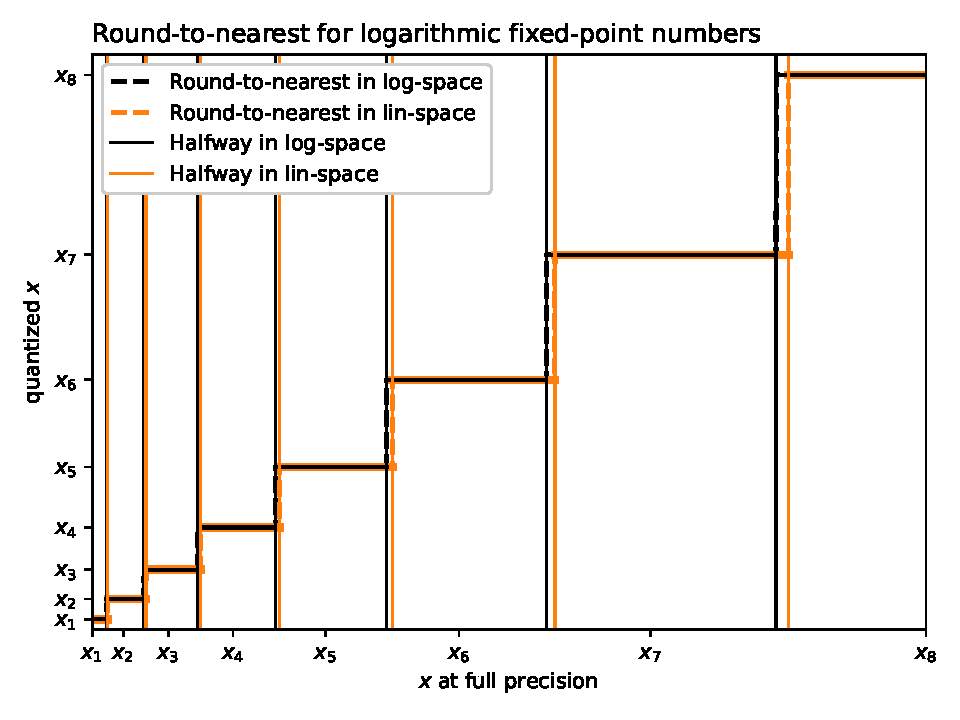
\includegraphics[width=1\textwidth]{Figures/methods/round_logquant.pdf}
	\caption{\textbf{Schematic to illustrate round-to-nearest in linear and logarithmic space for logarithmic
	fixed-point numbers.} Exact values $x$ at full precision are presented on the x-axis and their rounding
	to the logarithmically spaced representable numbers $x_1,...,x_8$ on the y-axis. Round-to-nearest in
	linear space will use the midpoints $\tfrac{x_i + x_{i+1}}{2}$ (arithmetic mean) as ties, round-to-nearest
	in logarithmic space uses the geometric mean $\sqrt{x_ix_{i+1}}$.}
	\label{fig:roundnearest_linlog}
\end{figure}

The rounding mode for logfixs is completed with an underflow at half the smallest representable number,
as for floats and posits (see section \ref{sec:roundnearest}) and no overflow, where $\pm maxpos$ is
returned instead as for posits. 

\subsection{Stochastic rounding}
\label{sec:stochastic_rounding}

The previously presented rounding modes are deterministic, such that a given exact value $x$ they always
return the same rounded value. This discards information contained in $x$ and two distinct exact values $x,y$
rounded to the same value cannot be distinguished anymore. In the following we will present one stochastic
rounding mode that can preserve some of this information at least in a statistical sense. 

For stochastic rounding, rounding of $x$ down to a representable number $x_1$ or up to $x_2$ occurs at probabilities
that are proportional to the distance between $x$ and $x_1$, $x_2$, respectively
\citep{Hohfeld1992,Muller2015,Gupta2015,Mikaitis2020,Croci2020}. Let $\delta$ be the distance between
$x_1,x_2$, $\delta = \vert x_2 - x_1 \vert$ then
\begin{equation}
\op{round}_{\op{stoch}}(x) =
\begin{cases}
x_1 \quad &\op{with~probability}\quad 1 - \delta^{-1}(x - x_1)  \\
x_2 &\op{with~probability}\quad  \delta^{-1}(x - x_1).
\end{cases}
\label{eq:stochround}
\end{equation}
This behaviour is illustrated in Fig. \ref{fig:methods_rounding_modes}. In case that $x$ is already identical with a
representable number no rounding is applied and the chance to obtain another representable number is zero.
In that sense stochastic rounding preserves the idempotence of the other deterministic rounding modes, i.e.
$\op{round}_{\op{stoch}}(\op{round}_{\op{stoch}}(x)) = \op{round}_{\op{stoch}}(x)$.

For $x$ being half way between two representable numbers, the chance of round up or round down is 50\%.
The introduced absolute rounding error for stochastic rounding is always at least as large as for round-to-nearest
and is larger when rounding away from the nearest representable number occurs. For $x$ just larger than $x_1$,
the probability that $x$ is rounded to $x_2$ is non-zero and the absolute rounding error can then be up to
$\pm \delta$, whereas for round-to-nearest the error is bounded by $\pm \tfrac{\delta}{2}$.  Although the average
absolute rounding error is therefore larger for stochastic rounding, the expected rounding error
decreases towards zero for repeated roundings
\begin{equation}
\lim_{N\to \infty}\frac{1}{N} \sum_i^N \op{round}_{\op{stoch}}(x) = x
\end{equation}
as follows by inserting Eq. \ref{eq:stochround}. Stochastic rounding is therefore exact in expectation. There are
other stochastic rounding modes, e.g. where the probability in Eq. \ref{eq:stochround} is $\tfrac{1}{2}$ in both
cases, which do not have this property. We will only discuss exact-in-expectation stochastic rounding in the
following.

\subsection{Efficient bitwise implementations}
\label{sec:bitwiseop}

The rounding modes from section \ref{sec:bitshave}, \ref{sec:roundnearest} and \ref{sec:stochastic_rounding} are 
implemented in binary using bitwise operations. The bitwise logical operations used are logical and (\&), or (|), and
exclusive or (xor, $\veebar$). Additionally, we will use the \emph{logical} bitshift operators $<< n$ and $>> n$ that shift the
bits by $n$ bit positions, push in \texttt{0}s and the bits pushed out are lost. For example, $\mathtt{01001011 >> 3 = 00001001}$
and $\mathtt{11011010 << 1 = 10110100}$. These are the default bitshift operations for unsigned integers, however,
for signed integers the right-bitshift operation $>>$ is an \emph{arithmetic} bitshift, which pushes in bits according to the
bit in the first bit position. For example, $\mathtt{1000 >> 1 = 1100}$ and $\mathtt{0111 >> 1 = 0011}$. This is motivated to
preserve the sign of negative integers (see section \ref{sec:int}, e.g. -8 $>>$ 1 = -4 and 8 $>>$ 1 = 4) and will be made use
of for the bitwise implementation of stochastic rounding. The algorithms presented here are implemented in a more general
form in the open-source packages \href{https://github.com/milankl/BitInformation.jl}{BitInformation.jl}
and \href{https://github.com/milankl/StochasticRounding.jl}{StochasticRounding.jl}.

\begin{figure}[tbhp]
\begin{lstlisting}[language=JuliaLocal, label=lst:bitshave, caption={\textbf{Bitwise implementation of bitshave, bitset and halfshave for
rounding to 7 mantissa bits.} Bitshave rounds a Float32 $x$ to $n_m = 7$ mantissa bits (equivalent to a BFloat16, but the tailing
bits remain stored) using the bitwise logical-and operation \&. For other number of mantissa bits to be retained the mask
\texttt{0xffff\_0000} has to be changed, e.g. \texttt{0xffff\_e000} will round to $n_m = 10$ mantissa bits. The function \texttt{reinterpret}
leaves the bits unchanged but changes the associated type. Bitset is implemented similar to bitshave but with the logical-or operation
$\vert$ which sets the tailing bits to \texttt{1}. Halfshave is similar to bitshave but the tailing bits are replaced by \texttt{100$...$0}.}]
function bitshave(x::Float32)
	ui = reinterpret(UInt32,x)
	ui &= 0xffff_0000	    # set last 16 bits to 0
	return reinterpret(Float32,ui)
end

function bitset(x::Float32)
	ui = reinterpret(UInt32,x)
	ui |= 0x0000_ffff    	# set last 16 bits to 1
	return reinterpret(Float32,ui)
end

function halfshave(x::Float32)
	ui = reinterpret(UInt32,x)
	ui &= 0xffff_0000    	# 1. shave last 16 bits to 1
	ui |= 0x0000_8000       # 2. set most significant tailbit to 1
	return reinterpret(Float32,ui)
end
\end{lstlisting}
\end{figure}
Bitshave, bitset and halfshave are easily implemented with the bitwise logical operations, given here as an example for rounding from
Float32 to BFloat16 (but preserving the tailbits, which would not be explicitly stored in most cases, Listing \ref{lst:bitshave}). Round-to-nearest
is more complicated to implement as the cases from Eq. \ref{eq:roundnearest} are implemented without if-clauses, efficiently using bitwise
operations (Listing \ref{lst:roundnearest}). This algorithm is adopted from the open-source package
\href{https://github.com/JuliaComputing/BFloat16s.jl}{BFloat16s.jl}.

\begin{figure}[tbhp]
\begin{lstlisting}[language=JuliaLocal, label=lst:roundnearest, caption={\textbf{Efficient round-to-nearest implemented with integer arithmetic.}
Example algorithm rounding Float32 to 7 mantissa bits as in Listing \ref{lst:bitshave}. Algorithm adapted from the open-source package
\href{https://github.com/milankl/BFloat16s.jl}{BFloat16s.jl}}]
function round_nearest(x::Float32)
    isnan(x) && return NaN32   # do not round NaNs
    ui = reinterpret(UInt32, x)
    # 1. check for even/odd of bit 16 with >> 16 & 1
    # 2. add either 0x7fff (even) or 0x8000 (odd) = +eps/2 with tie-to-even
    ui += 0x0000_7fff + ((ui >> 16) & 0x0000_0001)
    # 3. set tailing bits to 0 for rounding
    ui &= 0xffff_0000
    return reinterpret(Float32,ui)
end
\end{lstlisting}
\end{figure}
The general idea of implementing round-to-nearest is to add $\tfrac{\delta}{2}$ (half the distance $\delta$ between two representable numbers) before round-to-zero.
Ignoring the tie-to-even rule, Eq. \ref{eq:roundnearest} can also be written as $\op{round}_{\op{nearest}}(x) = \op{round}_{\op{to-zero}}(x + \tfrac{\delta}{2})$.
To account for the tie-to-even rule, one has to add just less than $\tfrac{\delta}{2}$ if $\op{round}_{\op{to-zero}}(x)$ even. Otherwise, adding $\tfrac{\delta}{2}$
to the tie will round up to the odd representable number, violating tie-to-even. In binary, using rounding Float32 to 7 mantissa bits as example, this is achieved
by checking the state of the least significant preserved bit. If $b_{16} = \mathtt{1}$ (bit 16, the 7th mantissa bit for Float32) then add \texttt{0x0000\_8000},
which corresponds to $\tfrac{\delta}{2}$, otherwise add \texttt{0x0000\_7fff}, which is just less than $\tfrac{\delta}{2}$ (see line 6 in Listing \ref{lst:roundnearest}).
Round-to-zero is then achieved as with bitshave in Listing \ref{lst:bitshave}, line 3). Note that the algorithm presented here uses integer arithmetic, such that
floating-point numbers are rounded without using floating-point arithmetic. We will take a similar approach for the implementation of stochastic rounding,
which is greatly simplified using integer arithmetic as discussed next.

\subsubsection{Stochastic rounding}

Implementing stochastic rounding directly from Eq. \ref{eq:stochround} requires the calculation of probabilities. It is more efficient however, to stochastically
perturb the exact value $x$ by adding a random number to it and then to deterministically round the result. However, implementing this idea with
floating-point arithmetic requires the random perturbation to be correctly scaled depending on the value $x$ itself. This involves several steps using
floating-point arithmetic, which will slow down the stochastic rounding compared to integer arithmetic-based implementations. We present an algorithm
that follows the same idea of randomly perturbing the exact value $x$, but in integer arithmetic which greatly simplifies stochastic rounding and 
avoids if-branching.

\begin{figure}[tbhp]
\begin{lstlisting}[language=JuliaLocal, label=lst:stochround, caption={\textbf{Efficient bitwise stochastic rounding with integer
arithmetic as implemented by StochasticRounding.jl} Example algorithm rounding Float32 to $n_f = 7$ mantissa bits as in Listing \ref{lst:bitshave}.
\texttt{rand(Int32)} creates 32 random bits with equal probabilities that are interpreted as Int32. Any pseudo random number generator can be used.
Line 5 returns zero if $\vert x \vert < \tfrac{1}{2}minpos$, $\mathtt{minpos\_half} = 2^{2-2^{n_e - 1} - (n_f + 1)} = \mathtt{0x0000\_8000}$ is a
constant defined globally (Eq. \ref{eq:float_all}).}]
function stochastic_round(x::Float32)
	rbits = rand(Int32)	# create random bits
	# branch off a return zero to avoid integer wrap-around
	# for values 0 < |x| < minpos/2 possibly producing NaN
	abs(x) < minpos_half && return zero(Float32)
	xi = reinterpret(Int32,x)
	# arithmetic bitshift >> to create a random integer that is in (-u/2,u/2)
	# always set last random bit to 1 via |1 to avoid creating -u/2
	xr = reinterpret(Float32,xi + ((rbits >> 16) | one(Int32)))
	return round_nearest(xr)
end
\end{lstlisting}
\end{figure}
While floats have a hybrid logarithmic-uniform distribution on the real axis, floats are uniformly distributed when interpreted as (signed) integers.
Hence, in line 9 of Listing \ref{lst:stochround} it is only necessary to arithmetic bitshift the random bits to the correct position and add them using
integer arithmetic, no further scaling is required. The arithmetic bitshift will create a random perturbation in $[-\tfrac{\delta}{2},\tfrac{\delta}{2})$
and the |1 operation is added to limit this range to $(-\tfrac{\delta}{2},\tfrac{\delta}{2})$ to avoid round down if $x$ is already perfectly representable.
Once the random perturbation is applied round-to-nearest will round down and up at correct probabilities. 

\section{Error norms}
\label{sec:error_norms}

To assess the impact of rounding errors, the absolute, mean, relative and decimal error are presented in the following.
The decimal error can be translated to the decimal precision, which is used to quantify and compare the precision of the
number formats from section \ref{sec:numbers}. 

\subsection{Absolute and mean error}
\label{sec:absmean_error}

The absolute, or linear error of an exact value $x$ and its approximation $\hat{x}$ (which is for example a representable number of
a finite-precision number format) is 
\begin{equation}
	\text{absolute error} = \vert x - \hat{x} \vert
	\label{eq:abserror}
\end{equation}
and therefore the $L_1$ distance between $x$ and $\hat{x}$ and preserves the unit of $x,\hat{x}$. The absolute error is invariant under addition,
$\vert (x+c) - (\hat{x} + c)\vert = \vert x - \hat{x} \vert$, such that using either Kelvin or degree Celsius yields the same absolute error.
However, the absolute is not invariant under scaling, such that using millimeter or meter will change also the unit of the absolute error,
$s^{-1}\vert x - \hat{x} \vert$ with scaling $s$, $x_s = sx, \hat{x}_s = s\hat{x}$. Assessing the absolute error of two arrays of numbers
the exact ones $X = (x_1,x_2,...,x_n)$ and the respective approximations $\hat{X} = (\hat{x}_1,\hat{x}_2,...,\hat{x}_n)$ yields $n$ 
absolute errors, hence an error distribution. The mean of such a distribution is the mean absolute error
\begin{equation}
	\text{mean absolute error} = \tfrac{1}{n} \sum_{i=1}^n \vert x_i - \hat{x}_i \vert
	\label{eq:meanabserror}
\end{equation}
and similarly the median, maximum or any other statistical property can be calculated.

In contrast, the mean error assesses the error in the respective means of the two arrays
\begin{equation}
	\text{mean error} = \tfrac{1}{n}\sum_{i=1}^n \hat{x}_i - \tfrac{1}{n}\sum_{i=1}^n x_i = \tfrac{1}{n} \sum_{i=1}^n \hat{x}_i - x_i
	\label{eq:meanerror}
\end{equation}
which can be both positive or negative. For example with $x_i \geq 0$ and $\hat{x}_i$ obtained via round-to-zero there is a
negative mean error (i.e. bias) as the mean after rounding is smaller than before. For round-away-from-zero the bias is
positive.

\subsection{Relative error}
\label{sec:relative_error}

The relative error assesses the absolute error relative to exact value. It is defined as
\begin{equation}
	\text{relative error} = \vert \frac{x - \hat{x}}{x} \vert
	\label{eq:relerror}
\end{equation}
and therefore dimensionless and invariant under scaling. The relative error does not discriminate sign changes, for example
the relative error for $x=1$ and $\hat{x} = 3$ or $\hat{x} = -1$ is identical: $\vert 1- 3 \vert = 2 = \vert 1 - (-1) \vert$. It is therefore
a less suitable error metric for non-negative variables like concentrations or precipitation. This issue is better addressed with
the decimal error, which is discussed next.

\begin{figure}[tbhp]
	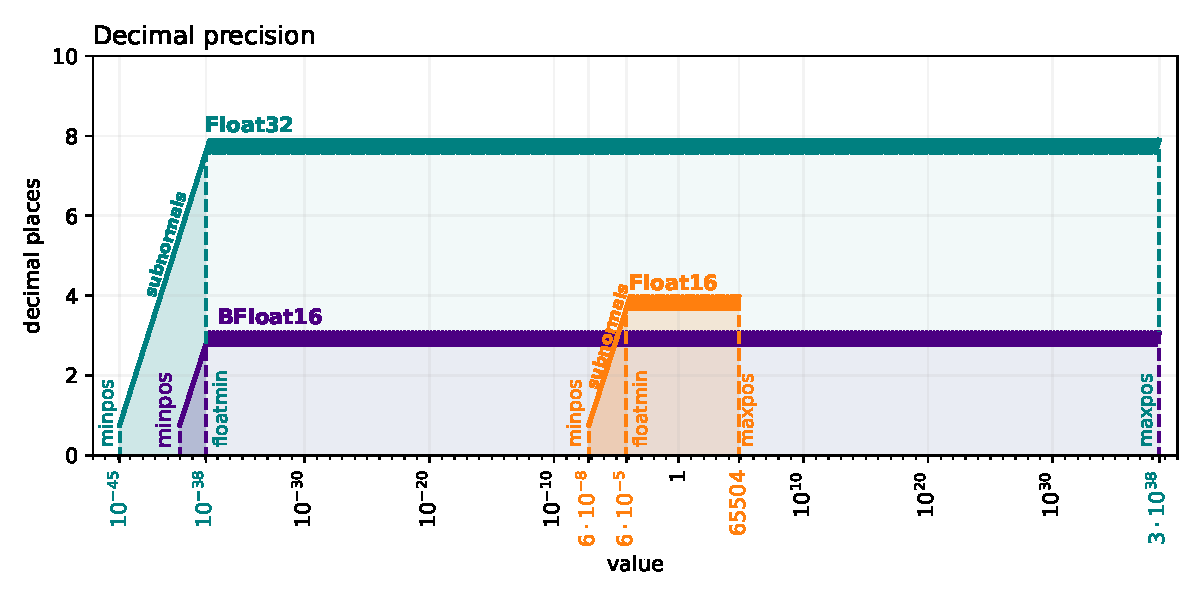
\includegraphics[width=1\textwidth]{Figures/methods/float32_16_bfloat_decprec.pdf}
	\caption{\textbf{Decimal precision of Float16, BFloat16 and Float32 over the range of representable numbers.}
	The decimal precision is worst-case, i.e. given in terms of decimal places that are at least correct after rounding
	(see section \ref{sec:decimal_precision}). The smallest representable number ($minpos$), the smallest normal number
	($floatmin$) and the largest representable number ($maxpos$) are denoted with vertical dashed lines (see section \ref{sec:floats}).
	The subnormal range is between $minpos$ and $floatmin$.}
	\label{fig:methods_decprec_floats}
\end{figure}

\subsection{Decimal error and precision}
\label{sec:decimal_precision}

The decimal error is here defined as
\begin{equation}
	\text{decimal error} = \begin{cases}
						0 &\text{for } x = \hat{x} = 0 \\
						\infty &\text{for } \op{sign}(x) \neq \op{sign}(\hat{x}) \\
						\vert \log_{10}\left( \frac{x}{\hat{x}} \right) \vert &\text{else.}
					\end{cases}
	\label{eq:decerror}
\end{equation}
and therefore the absolute error in logarithmic space
$\vert \log_{10}(\tfrac{x}{\hat{x}}) \vert = \vert \log_{10}(x) - \log_{10}(\hat{x}) \vert$ unless $x = \hat{x} = 0$.
The decimal error quantifies the orders of magnitude an approximation $\hat{x}$ is away from the exact value $x$,
for example $x = 1$ and $\hat{x} = 10$ yields a decimal error of 1, and so does $\hat{x} = \tfrac{1}{10}$. Based on
the decimal error the decimal precision is defined for $\op{sign}(x) = \op{sign}(\hat{x})$ and $x \neq 0, \hat{x} \neq 0$ 
as \citep{Gustafson2017a,Klower2019a}
\begin{equation}
\op{decimal} \op{precision} = -\log_{10} \vert \log_{10} \left( \frac{x}{\hat{x}} \right) \vert
\end{equation}
The decimal precision quantifies the number of decimal places that are correct when using $\hat{x}$ as an approximate
to $x$. For example, $x = \pi$ and $\hat{x} = 3.14$ yields a decimal precision of $3.66...$, as the three explicit decimal
digits $3,1,4$ agree and the following implicit 0 digits in $\hat{x} = 3.1400...$ are close to the exact digits $159...$ in $3.14{\color{pregime}159}...$

The decimal precision approaches infinity when the approximation $\hat{x}$ approaches the exact result $x$ (where the
decimal error drops to 0). For the round-to-nearest rounding mode, the decimal precision has a minimum
at the geometric mean $\sqrt{\hat{x}_1\hat{x}_2}$ in between two representable numbers $\hat{x}_1,\hat{x}_2$. 
This minimum defines the \emph{worst-case} decimal precision, i.e. the decimal precision when the rounding error
is maximised. The worst-case decimal precision is the number of decimal places that are at least correct after rounding
\citep{Gustafson2017a}. So while the decimal precision of a given number format over the whole
range of representable numbers is of interest, it is dependent on the exact location of representable numbers not just
the spacing in between. In contrast, the worst-case decimal precision over the whole range of representable numbers
is a more useful metric to assess the provided precision of a number format. In the following we will refer to the
worst-case decimal precision simply as decimal precision.

Fig. \ref{fig:methods_decprec_floats} compares the decimal precision for the three floating-point formats Float32, Float16
and BFloat16. Due to the exponent bits, the decimal precision is approximately constant over the normal range of 
floats for each format. It is not exactly constant as the mantissa bits are uniformly distributed between two powers of 2
(Eq. \ref{eq:float}), hence the decimal precision for these increases towards the larger of the two powers of 2. This
increase causes a sawtooth wave with a wavelength that is exactly the distance between two consecutive powers
of two. The minimum of this sawtooth wave is reached when the spacing doubles between floats larger than the
next power of 2. A zoomed-in version of Fig. \ref{fig:methods_decprec_floats} is Fig. \ref{fig:methods_decimal_precision_all},
which will later discuss the decimal precision of other formats.

Subnormal floats are uniformly distributed, such that their decimal precision drops towards 0 between
$floatmin$ and $minpos$. Float32 has a decimal precision of at least 7.6 decimal places over more than 80 orders
of magnitude (Table \ref{tab:formats}). Due to only 7 mantissa bits with BFloat16, this format has a much lower
decimal precision of 2.8 decimal places. One can therefore not expect more than 3 decimal digits to be correct
when using BFloat16 for calculations. While BFloat16 largely preserves the dynamic range of Float32, Float16
uses 10 mantissa bits, reducing the dynamic range to 12 orders of magnitude. Using 3 bits for the mantissa instead
of the exponent, Float16 reaches a decimal precision of 3.7. 

\begin{figure}[tbhp]
	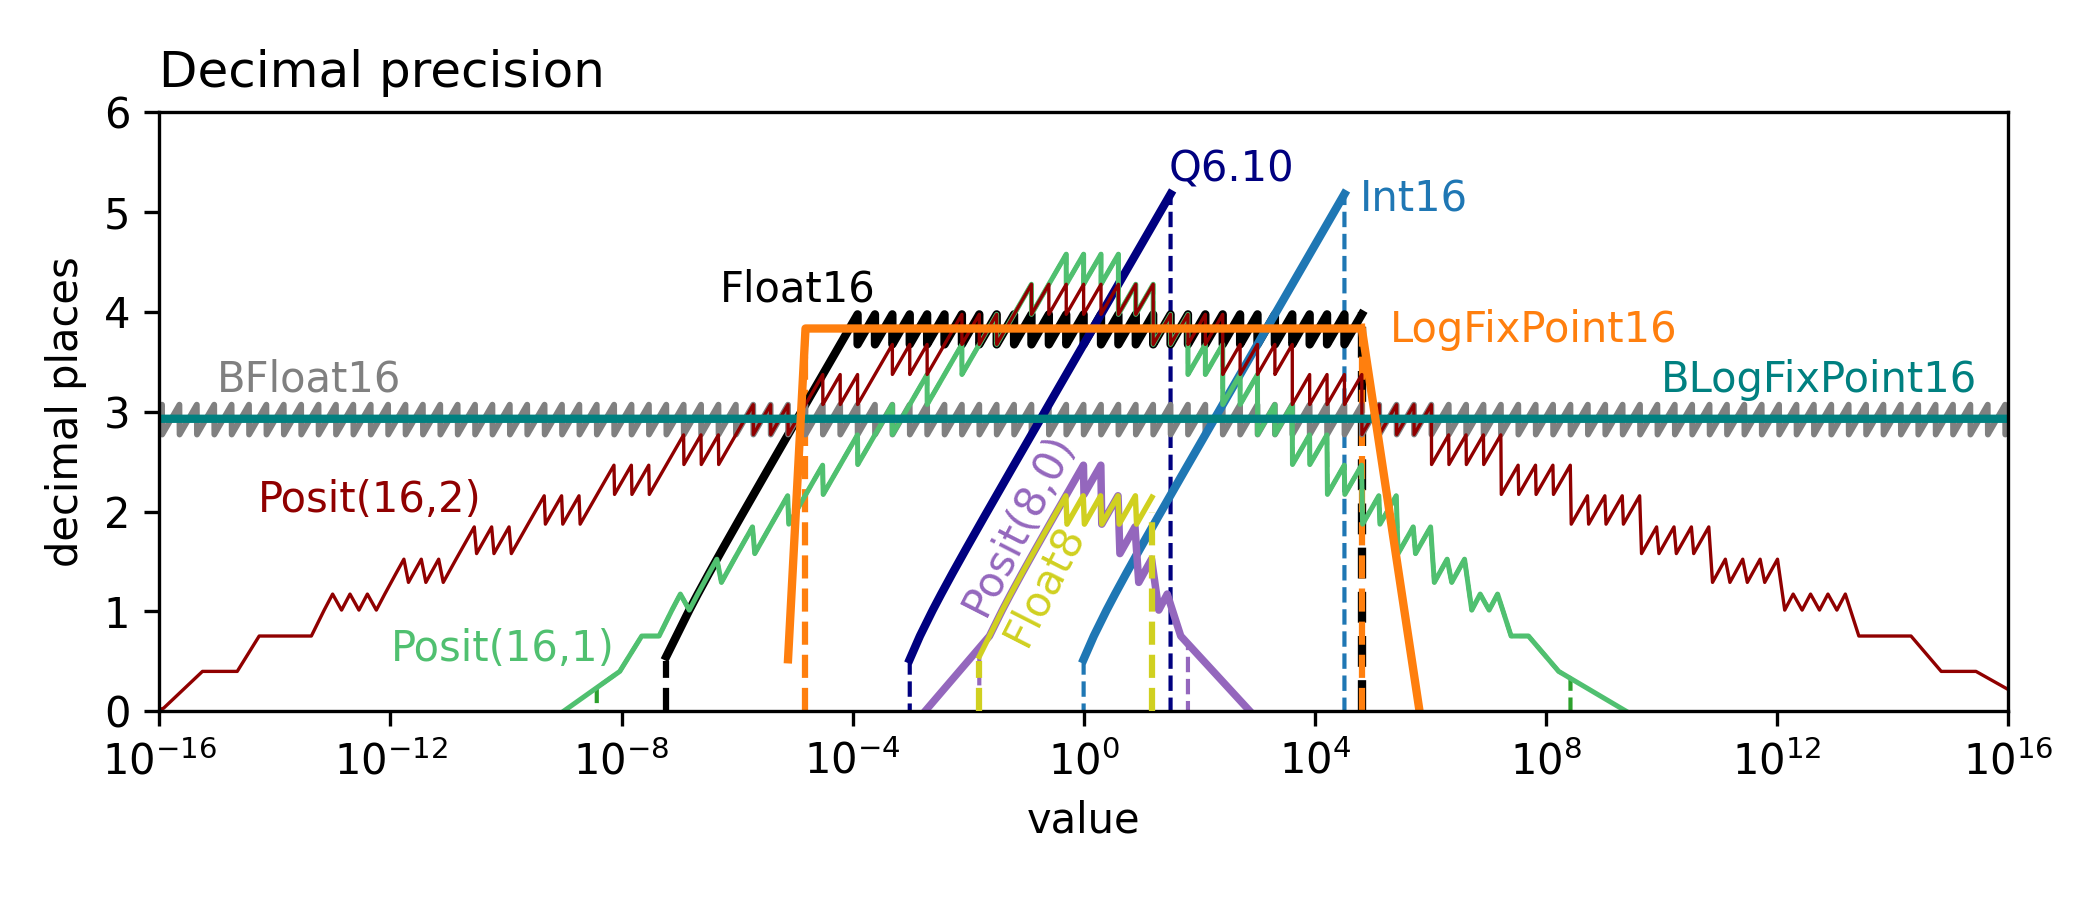
\includegraphics[width=1\textwidth]{Figures/methods/decimal_precision_all.png}
	\caption{\textbf{Decimal precision of various 8 and 16-bit number formats.} The number formats are described
	in more detail in Table \ref{tab:formats}. The decimal precision is worst-case, i.e. given in terms of decimal places
	that are at least correct after rounding (see section \ref{sec:decimal_precision}). Vertical dashed lines indicate
	the range of representable numbers $(minpos,maxpos)$, respectively. BFloat16 and BLogFixPoint16 have 
	representable range outside the figure limits, see Fig. \ref{fig:methods_decprec_floats}.}
	\label{fig:methods_decimal_precision_all}
\end{figure}

The decimal precision of posits consists of a similar sawtooth wave as for floats as they share the same definition 
for the mantissa/fraction bits. However, for every power of $useed$ away from $1$ there is one bitposition less
available for the mantissa. Consequently, posits have a pyramid-like shape in the decimal precision, whereby
highest precisions are reached for the power of $useed$ (e.g. $useed = 4$ for 1 exponent bit) centred on 1.
The gradually lower precision away from 1, allows posits to have both a high precision at 1 and at the same time
a wide dynamic range. The no-overflow rounding mode can be seen as the precision does not immediately drop
to negative infinity outside the dynamic range for posits.

The logarithmic fixed-point number formats LogFixPoint16 and BLogFixPoint16 have a perfectly flat decimal precision
of about 4 and 3 decimal places, respectively, due to the logarithmic spacing of the representable numbers.
The precision drops quickly, but not immediately, to zero outside of the dynamic range due to the no-overflow rounding
mode adopted from posits. However, the decimal precision for LogFixPoint16 and BLogFixPoint16 only applies to
operations such as conversion, addition and subtraction. For multiplication, division, power of 2 and square root 
the decimal precision is infinity, as these arithmetic operations map perfectly onto another logfix number for all arguments,
unless an underflow or overflow occurs (section \ref{sec:logfixs}).

The decimal precision of 16-bit signed integers Int16 is negative infinity for any number below 0.5 (round to 0) and
increases to the largest representable integer $maxpos = 2^{15} - 1 =  32767$. In that sense, using signed integers for scientific
computing is tricky as most calculations should be placed near $maxpos$ for increased precision, but a result beyond
$maxpos$ will yield desastrous results to the the wrap-around behaviour of integers (section \ref{sec:int}).
Similar conclusions hold for the fixed-point format Q6.10, as the decimal precision is simply shifted towards smaller
numbers by a factor of $\tfrac{1}{2}$ for each additional fraction bit.

\section{Code composability through type flexibility}
\label{sec:type_flexible}

The various number formats of the previous sections have to be emulated in software to use them in simulations, as only
Float32 and Float64 are widely supported on hardware. Float16 is an exception as it is emulated in all chapters but
chapter \ref{chap:hardware}, which explicitly describes the usage of hardware-accelerated Float16. We therefore
describe in the following the necessary programming paradigms to efficiently implement algorithms in a way
that any (custom) number format can be used, whether hardware-accelerated or not. This type flexibility can also
be exploited for number formats that analyse the code during execution, which is described in section \ref{sec:analysis_number_formats}.

\subsection{A type-flexible programming paradigm}

The Julia programming language provides several programming paradigms that facilitate the use of arbitrary number formats
without the need to rewrite an algorithm \citep{Bezanson2017}. As this is an essential feature of Julia and extensively made 
use of in several chapters, we briefly outline the benefits of Julia by computing the harmonic sum
$\sum_{i=1}^\infty \tfrac{1}{i}$ with various number formats as an example. Analytically the harmonic sum diverges, but with
finite-precision arithmetic several issues arise: With an increasing sum the precision is eventually lower than required to
represent the increment of the next summand. The integer i as well as its inverse $\tfrac{1}{i}$ have to be representable
in a given number format, and are also subject to rounding errors.

\begin{figure}[tbhp]
\begin{lstlisting}[language=JuliaLocal, label=lst:harmonic_sum, caption={\textbf{A type-flexible function calculating the harmonic sum in Julia.}
The number format is passed on as type in the first argument. The syntax \texttt{where T} triggers a separate compilation for every number
format. The function \texttt{harmonic\_sum} is type-stable as all types inside the function are declared and therefore unambiguous to the
compiler.}]
function harmonic_sum(::Type{T},steps::Int=2000) where T

    s = zero(T)     # partial sum, start with zero-element of type T
    oone = one(T)   # numerator of every fraction, one-element of type T

    for i in 1:steps
        s_old = s
        s += oone/convert(T,i)  # s = s + 1/i, harmonic sum

        if s == s_old           # check for convergence
            print((Float64(s),i))
            break
        end
    end
end
\end{lstlisting}
\end{figure}

The function \texttt{harmonic\_sum} takes 2 positional arguments, whereby the second is optional and just prevents an
infinite loop (Listing \ref{lst:harmonic_sum}). As the first argument the function takes a type \texttt{T}, which can be a
number format or any other, possibly custom, type in Julia. The syntax \texttt{where T} triggers a separate compilation
for every type \texttt{T} that is provided as the first argument. Julia hereby makes use of its just-in-time (JIT) compiler,
which automatically compiles a function at first execution. It relies thereby on \emph{multiple-dispatch} which is a
programming paradigm whereby all types of the arguments are assessed to determine which (possibly already compiled)
version of a function to execute. Multiple-dispatch therefore avoids overloading of functions, as several functions
can exist in parallel, as long as they are defined for different types (and the most type-specific version is chosen in
case functions are defined for super and subtypes).

The function is \texttt{harmonic\_sum} is type-stable, as the types of all variables are either internally declared (e.g.
\texttt{i}, the counter of the loop is always an integer) or follow directly from the provided types in the arguments.
Therefore, writing abstractly \texttt{s = zero(T)} to obtain the zero-element of type \texttt{T} instead of \texttt{s = 0}
is important to avoid implicit conversions between types. The function is \texttt{harmonic\_sum} is also type-flexible,
as it can be executed with every type \texttt{T} that has the following functions defined: \texttt{zero(T), one(T)}, addition,
division, comparison (\texttt{==} in line 10) conversion from integer (\texttt{convert(T,i)} in line 8) and to Float64.
For example, \texttt{zero(::Type\{Posit8\}) = reinterpret(Posit8,0x00)} to define the zero-element for 8-bit posits, or
\texttt{+(x::LogFixPoint16,y::LogFixPoint16) = ...} to define the addition between LogFixPoint16s.

These features of Julia allow for \emph{code composability}. As the function \texttt{harmonic\_sum} is abstractly written
to allow for type flexibility it does not know about any (possibly custom) number format, such as posits or logfixs.
On the other hand, we can define a custom number format including its arithmetic and other functions
(e.g. \texttt{zero(T)}) that does not know about the function \texttt{harmonic\_sum}. In essence, while both codes
are completely independent (and possible defined in separate packages), they are composable, meaning they can
be executed together. The function \texttt{harmonic\_sum} therefore has to be defined only once, and does not have
to be  changed or rewritten for other formats.

\begin{figure}[tbhp]
\begin{lstlisting}[language=JuliaLocal, label=lst:harmonic_sum2, caption={\textbf{Executing \texttt{harmonic\_sum} with different
number formats in the Julia shell.} The number format is passed on as an argument, causing the function \texttt{harmonic\_sum}
to be compiled and executed with that format. Depending on the precision of the number format, the harmonic sum converges
after 65 (BFloat16) to 1024 elements (Posit16).}]
julia> using SoftPosit, BFloat16s, LogFixPoint16s   # load number formats
julia> LogFixPoint16s.set_nfrac(10)                 # set to 10 fraction bits
julia> harmonic_sum(Float16)
(7.0859375, 513)            # converged to 7.09... after 513 elements

julia> harmonic_sum(BFloat16)
(5.0625, 65)                # converged to 5.06... after 65 elements

julia> harmonic_sum(Posit16)
(7.77734375, 1024)          # converged to 7.78... after 1024 elements

julia> harmonic_sum(LogFixPoint16)
(6.851249694824219, 432)    # converged to 6.85... after 432 elements
\end{lstlisting}
\end{figure}

The harmonic sum converges after 513 elements when using Float16 (Listing \ref{lst:harmonic_sum2}). The precision of BFloat16
is so low that the sum already converges after 65 elements, as the addition of the next term $\tfrac{1}{66}$ is rounded back to
$5.0625$. The addition of small terms to values of size $\mathcal{O}(1)$ is one of the major challenges with low-precision arithmetic,
(section \ref{sec:swm_mixed} and \ref{sec:compensated_time_integration}). Using Posit16, the sum converges only after 1024 terms,
due to the higher decimal precision of posits between 1 and 8. The precision of LogFixPoint16 is similar to Float16, and the sum
converges after 432 elements.

\subsection{Analysis number formats}
\label{sec:analysis_number_formats}

The type flexibility and code composability in Julia can be further extended by designing a custom number format that executes
additional code than just returning the result when an arithmetic operations is called. If we are interested to understand why and
how the harmonic sum converges with low precision number formats, we could alter \texttt{harmonic\_sum} directly, however,
for many larger algorithms, nested in a large amount of functions, this might be unfeasible or inefficient. Julia's code
composability offers another high-level way that is illustrated in the following.

We create a new custom number format by defining a new type Float16print (Listing \ref{lst:float16print}, line 1-3), which behaves as Float16
but we explicitly alter the definition of the addition for two Float16print values to execute additional code that helps to analyse the
function \texttt{harmonic\_sum}. Here, we add a print statement to obtain information on the numbers that are calculated within 
\texttt{harmonic\_sum}, without changing \texttt{harmonic\_sum} itself. In general, the arithmetic operations can be altered in many ways,
and more specific implementations of analysis number formats are presented in section \ref{sec:scale_sherlogs}.

\begin{figure}[tbhp]
\begin{lstlisting}[language=JuliaLocal, label=lst:float16print, caption={\textbf{Minimal example of the definition of a new custom analysis
number format \texttt{Float16print} in Julia.} The number format behaves like Float16 and defines all operations needed for \texttt{harmonic\_sum}
but the addition is extended with a \texttt{print} statement that helps to analyse code without changing \texttt{harmonic\_sum} itself.}]
struct Float16print      # define a custom type called Float16print
    float16::Float16     # that contains only a Float16
end

# extend the zero and one functions for Float16print (same as for Float16)
Base.zero(::Type{Float16print}) = Float16print(zero(Float16))
Base.one(::Type{Float16print}) = Float16print(one(Float16))

# define division (/) for Float16print as for Float16
Base.:(/)(x::Float16print,y::Float16print) =
					Float16print(x.float16 / y.float16)

# define addition (+) for Float16print as for Float16 but also print result
function Base.:(+)(x::Float16print,y::Float16print)
     z = x.float16 + y.float16     # unpack into float16, perform addition
     println(z)                    # add any aditional analysis code here
     return Float16print(z)
end

# define conversion from Integer and to Float64 as for Float16
Base.convert(::Type{Float16print},i::Int64) = Float16print(Float16(i))
Base.Float64(x::Float16print) = Float64(x.float16)
\end{lstlisting}
\end{figure}

While the application here is rather simple, it shows how custom analysis number format will change the compilation of a function. Here,
Julia's compiler will create an compiled version of \texttt{harmonic\_sum} that contains a \texttt{print} statement after
every addition, by doing so the two codes of Listing \ref{lst:harmonic_sum} and \ref{lst:float16print} are composed allowing the user
to interfere with pre-existing algorithms on a high-level basis, e.g. no compiler knowledge is necessary.a

\begin{figure}[tbhp]
\begin{lstlisting}[language=JuliaLocal, label=lst:harmonic_sum_float16print, caption={\textbf{Analysing the function \texttt{harmonic\_sum} with the
new custom number format \texttt{Float16print}.} Executing \texttt{harmonic\_sum} with \texttt{Float16print} triggers a \texttt{print} statement
on every addition, i.e. after every term of the harmonic sum, but any other additional code can be executed too. Analysis number formats can
be used to investigate even complicated algorithms without explicitly changing them.}]
julia> harmonic_sum(Float16print)
1.0
1.5
1.833
...
7.082
7.086
7.086
(7.0859375, 513)
\end{lstlisting}
\end{figure}

As a result, Listing \ref{lst:harmonic_sum_float16print} shows how the first elements of the harmonic sum $1 + \tfrac{1}{2} + \tfrac{1}{3} + ...$ are added,
and how the sum stagnates at $7.086$. The next term $\tfrac{1}{514}$ cannot be added as it is less than half the distance to the next representable number,
and therefore round back to $7.086$.

\section{Information theory}
\label{sec:information}

The following sections introduce fundamental ideas of information theory and how they can be applied to analyse the information contained in the bits
of binary numbers that are used for weather and climate computing. A more specific discussion on the bitwise real information content analysed for
atmospheric data in chapter \ref{chap:compression} is found in section \ref{sec:compression_methods_information_content}.

\subsection{Entropy}
\label{sec:entropy}

Information entropy is a quantity that measures the amount of information contained in a random variables \citep{Shannon1948,MacKay2003}.
A random variable with $n$ discrete outcomes at chances $p_i \geq 0, i = 1,...,n$ has a probability mass function determined by $p_i$ for which
the information entropy $H$ is calculated as
\begin{equation}
	H = - \sum_i^n p_i \log_b(p_i)
	\label{eq:entropy}
\end{equation}
The base $b$ of the logarithm defines the unit of entropy. In the following chapters we will exclusively use $b=2$ such that the unit of information
is given in bits.

Considering the flip of a coin with equal probabilities $p_1=p_2=\tfrac{1}{2}$ (e.g. for $i=1$ the outcome is \emph{tail}, and for $i=2$ it is \emph{head})
as a first example how to interpret information entropy. Before the coin is flipped, it is known that the outcome is equally likely tail or head. After flipping the
coin the outcome is observed and we are equally surprised about either outcome. Given our knowledge of the probabilities we had an equal expectation
for tail or head and so the uncertainty of the outcome is maximised. Applying Eq. \ref{eq:entropy} yields an entropy of 1 bit, which corresponds to
representing head and tail with \texttt{0} and \texttt{1} such that a sequence of 8 coin flips can be recorded as, for example, \texttt{10110100}.
The observation of the outcome of every coin flip adds another bit to the sequence.

Assume now that the coin is bent, such that its probabilities change to $p_1 = \tfrac{1}{10}$ and $p_2 = \tfrac{9}{10}$. Now we should expect the outcome
of a flip to be head, as it is much more likely than tail. Hence, we would be surprised if the outcome was indeed tail given its probability. In this sense
the information entropy can be interpreted as the average surprise when observing outcomes. In 9 out of 10 cases we would not be surprised as the
outcome is head as we should expect, but in 1 out of 10 cases we would be surprised --- the rarer the event the larger the surprise. The entropy of such
a bent coin flip is calculated to be about $0.47$ bit, hence less than half of the coin flip with equal probabilities. Observing the coin flip conveys here
less information as in most cases we already know what the outcome will be. Recording several coin flips with \texttt{0} and \texttt{1} as before
will yield a sequence, for example, like \texttt{0000100000000100...} which consists mostly of \texttt{0}s.

The entropy of a random variable is maximised for a uniform distribution, i.e. all outcomes are equally likely (see Eq. \ref{eq:entropy}). For $n$
possible outcomes the maximum entropy is then $\log_2(n)$ in units of bits. The coin flip with equal probabilities therefore has maximum
entropy, meaning that the prior knowledge of its probabilities does not provide a mean to predict the next outcome. In that sense, observing
the next outcome provides exactly 1 bit of information. In contrast, the flip of a bent coin does not have maximum entropy. Shannon's source
coding theorem \citep{Shannon1948} therefore says that there is a way to encode a sequence like \texttt{0000100000000100...} (as
observed for the bent coin) with less than 1 bit per coin flip. In fact, its entropy of 0.47 bit is a lower limit on the average number of bits needed
to encode such a sequence. Intuitively, one may think of an encoding which only stores the number of flips until the next \texttt{1} (i.e. head)
is observed, here $5,9,...$. Finding an encoding that requires less storage is the subject of lossless compression algorithms, which
aim to remove redundancies (here long sequences of \texttt{0}s) until an encoding is found that itself approaches maximum entropy.

\subsection{Bitpattern entropy}
\label{sec:bitpattern_entropy}

An $n$-bit number format has $2^n$ bitpatterns available to encode a real number. The bitpattern entropy is the
Shannon information entropy $H$, in units of bits \citep{Shannon1948}, calculated from the probability of each bitpattern 
	\begin{equation}
	H = - \sum_{i=1}^{2^n} p_i \log_2(p_i)
	\end{equation}
For most data arrays, not all bitpatterns are used at uniform probability for which $p_i = 2^{-n}$, which maximises the entropy
to $H = \log_2(2^n) = n$. The difference $n-H$ between maximum entropy $n$ and the actual entropy $H$ is denoted as free
entropy and can be interpreted as the number of bits that are effectively unused in the encoding of a data array into the
respective number format. For example, a data array of signed integers that is uniform in the positive range, but does not
contain negative integers will have a free entropy of 1 bit, as the sign bit is unused.

Floating-point numbers can never have a maximum entropy as their encoding is not a bijective function. While one could argue
that encoding both +0 and -0 with distinct bitpatterns is bijective ($\tfrac{1}{-0} = -\infty \neq \infty = \tfrac{1}{0}$ in float arithmetic),
many bitpatterns are used to encode NaN (see Eq. \ref{eq:float_all}), violating bijection. In practice, the free entropy resulting
from this redundancy is negligible. Even for Float8 with 12.5\% of bitpatterns representing NaR (Table \ref{tab:formats}) the 
resulting free entropy is 0.2 bit, reducing the maximum entropy of 8 bit to 7.8 bit. In contrast, using Float64 to represent 
numbers in the range of [256,512) (similar to for example air or water temperature on Earth in Kelvin) has an entropy of at 
most 52 bit compared to the 64 available bits as the sign and exponent bits are unused. Furthermore, such a data array
would need to have at least $2^{52} \approx 10^{15.6}$ entries to reach maximum entropy in 52 bits. This corresponds to
a theoretical array size of 36 Petabyte, which is far beyond typical array sizes. From an entropy perspective, using 64-bit number
formats are therefore a very inefficient way to encode real numbers into bits. Nevertheless, this entropy inefficiency allows
Float64 calculations to have minimal rounding errors.

\subsection{Mutual information}
\label{sec:mutual_information}

In the previous section, the 








